%        File: pres.tex
%     Created: Tues June 19 07:00 AM 2012 C
%
%\documentclass[11pt,handout]{beamer}
\documentclass[9pt]{beamer}
% for beamer arrows
\usepackage{tikz}
\usetikzlibrary{arrows,shapes}



\usepackage{graphicx}
\usepackage{booktabs} % nice rules for tables
\usepackage{microtype} % if using PDF
\usepackage{bigints}
\newcommand{\units}[1] {\:\text{#1}}%
\newcommand{\SN}{S$_N$}%{S$_\text{N}$}%{$S_N$}%
\DeclareMathOperator{\erf}{erf}
\setbeamertemplate{caption}[numbered]

\usetheme[white]{Wisconsin}
%\title[short title]{long title}
\title[Cyclus and Cyder]{ Cyclus and Cyder : Open Source Tools for Fuel Cycle and Repository Analysis}
\title[Key Disposal Processes and Parameters]{ Key Processes and Parameters in a Generic Clay Disposal System Model}
%\subtitle[short subtitle]{long subtitle}
\subtitle[ANS2012]{2012 American Nuclear Society Winter Meeting, San Diego} 
%\author[short name]{long name}
\author[Kathryn Huff]{Kathryn D.~Huff$^{1,2}$ \& W. Mark Nutt$^2$}
%\date[short date]{long date}
\date[11.13.2012]{November 13, 2012}
%\institution[short name]{long name}
\institute[UW-Madison]{$^1$University of Wisconsin-Madison \& $^2$Argonne National Laboratory}
%page numbers
\setbeamertemplate{footline}[page number]
%Those icons in the references are terrible looking
\setbeamertemplate{bibliography item}[text]

%%%%%%%%%%%%%%%%%%%%%%%%%%%%%%%%%%%%%%%%%%%%%%%%%%%%%%%%%%%%%
\usepackage[acronym,toc]{glossaries}
\newacronym{MIT}{MIT}{the Massachusettes Institute of Technology}
\newacronym{UW}{UW}{University of Wisconsin}
\newacronym{US}{US}{United States}
\newacronym{IAEA}{IAEA}{International Atomic Energy Agency}
\newacronym{SNF}{SNF}{spent nuclear fuel}
\newacronym{HLW}{HLW}{high level waste}
\newacronym{FEHM}{FEHM}{Finite Element Heat and Mass Transfer}
\newacronym{DOE}{DOE}{Department of Energy}
\newacronym{GENIUSv2}{GENIUS}{Global Evaluation of Nuclear Infrastructure Utilization Scenarios, Version 2}
\newacronym{CNERG}{CNERG}{Computational Nuclear Engineering Research Group}
\newacronym{GDSM}{GDSM}{Generic Disposal System Model}
\newacronym{GDSE}{GDSE}{Generic Disposal Sytem Environment}
\newacronym{GPAM}{GPAM}{Generic Performance Asessment Model}
\newacronym{FEPs}{FEPs}{Features, Events, and Processes}
\newacronym{EBS}{EBS}{Engineered Barrier System}
\newacronym{EDZ}{EDZ}{Excavation Disturbed Zone}
\newacronym{YMR}{YMR}{Yucca Mountain Repository Site}
\newacronym{EPA}{EPA}{Environmental Protection Agency}
\newacronym{PEI}{PEI}{Peak Environmental Impact}
\newacronym{VISION}{VISION}{the Verifiable Fuel Cycle Simulation Model}
\newacronym{NUWASTE}{NUWASTE}{Nuclear Waste Assessment System for Technical Evaluation}
\newacronym{NWTRB}{NWTRB}{Nuclear Waste Technical Review Board}
\newacronym{OCRWM}{OCRWM}{Office of Civillian Radioactive Waste Management}
\newacronym{UFD}{UFD}{Used Fuel Disposition}
\newacronym{DYMOND}{DYMOND}{Dynamic Model of Nuclear Development }
\newacronym{DANESS}{DANESS}{Dynamic Analysis of Nuclear Energy System Strategies}
\newacronym{CAFCA}{CAFCA}{ Code for Advanced Fuel Cycles Assessment }
\newacronym{ORION}{ORION}{O..}
\newacronym{NFCSim}{NFCSim}{Nuclear Fuel Cycle Simulator}
\newacronym{COSI}{COSI}{Commelini-Sicard}
\newacronym{FCT}{FCT}{Fuel Cycle Technology}
\newacronym{SWF}{SWF}{Separations and Waste Forms}
\newacronym{FCO}{FCO}{Fuel Cycle Options}
\newacronym{RDD}{RD\&D}{Research Development and Design}
\newacronym{WIPP}{WIPP}{Waste Isolation Pilot Plant}
\newacronym{ANDRA}{ANDRA}{Agence Nationale pour la gestion des D\'echets RAdioactifs, the French National Agency for Radioactive Waste Management}
\newacronym{TSM}{TSM}{Total System Model}
\newacronym{LANL}{LANL}{Los Alamos National Laboratory}
\newacronym{INL}{INL}{Idaho National Laboratory}
\newacronym{ANL}{ANL}{Argonne National Laboratory}
\newacronym{SNL}{SNL}{Sandia National Laboratory}
\newacronym{LBNL}{LBNL}{Lawrence Berkeley National Laboratory}
\newacronym{LLNL}{LLNL}{Lawrence Livermore National Laboratory}
\newacronym{NAGRA}{NAGRA}{National Cooperative for the Disposal of Radioactive Waste}
\newacronym{CUBIT}{CUBIT}{CUBIT Geometry and Mesh Generation Toolkit}
\newacronym{CSNF}{CSNF}{Commercial Spent Nuclear Fuel}
\newacronym{DSNF}{DSNF}{DOE Spent Nuclear Fuel}
\newacronym{MTHM}{MTHM}{Metric Ton of Heavy Metal}
\newacronym{HTGR}{HTGR}{High Temperature Gas Reactor}
\newacronym{TRISO}{TRISO}{Tristructural Isotropic}
\newacronym{MA}{MA}{Minor Actinide}
\newacronym{CEA}{CEA}{Commissariat a l'Energie Atomique et aux Energies Alternatives}
\newacronym{SKB}{SKB}{Svensk Karnbranslehantering AB}
\newacronym{SINDAG}{SINDA{\textbackslash}G}{Systems Improved Numerical Differencing Analyzer $\backslash$ Gaski}
%\newacronym{<++>}{<++>}{<++>}

\makeglossaries


\begin{document}
%%%%%%%%%%%%%%%%%%%%%%%%%%%%%%%%%%%%%%%%%%%%%%%%%%%%%%%%%%%%%
%% From uw-beamer Here's a handy bit of code to place at 
%% the beginning of your presentation (after \begin{document}):
\newcommand*{\alphabet}{ABCDEFGHIJKLMNOPQRSTUVWXYZabcdefghijklmnopqrstuvwxyz}
\newlength{\highlightheight}
\newlength{\highlightdepth}
\newlength{\highlightmargin}
\setlength{\highlightmargin}{2pt}
\settoheight{\highlightheight}{\alphabet}
\settodepth{\highlightdepth}{\alphabet}
\addtolength{\highlightheight}{\highlightmargin}
\addtolength{\highlightdepth}{\highlightmargin}
\addtolength{\highlightheight}{\highlightdepth}
\newcommand*{\Highlight}{\rlap{\textcolor{HighlightBackground}{\rule[-\highlightdepth]{\linewidth}{\highlightheight}}}}
%%%%%%%%%%%%%%%%%%%%%%%%%%%%%%%%%%%%%%%%%%%%%%%%%%%%%%%%%%%%%
%%--------------------------------%%
\frame{
\titlepage
}
%%--------------------------------%%
\AtBeginSection[]{
\begin{frame}[c]
  \frametitle{Outline}
  \tableofcontents[currentsection]
\end{frame}
}

%%--------------------------------%%
%%--------------------------------%%

%%%%%%%%%%%%%%%%%%%%%%%%%%%%%%%%%%%%%%%%%%%%%%%%%%%%%%%%%%%%%%%%%%%%%%%%%%%%%%%%
  
\section{Introduction}
\begin{frame}[c]
  \frametitle{Clay Generic Disposal System Model}
Sensitivity analysis based on the detailed computational \textbf{Clay 
  \gls{GDSE}} developed by the \gls{UFD} campaign \cite{clayton_generic_2011}.  
  was performed with respect to various \textbf{key processes and parameters} 
  affecting long-term post-closure performance of geologic repositories in 
  \textbf{clay} media.

\end{frame}

\begin{frame}[c]
  \frametitle{Clay Generic Disposal System Model}
     \begin{figure}[h!]
         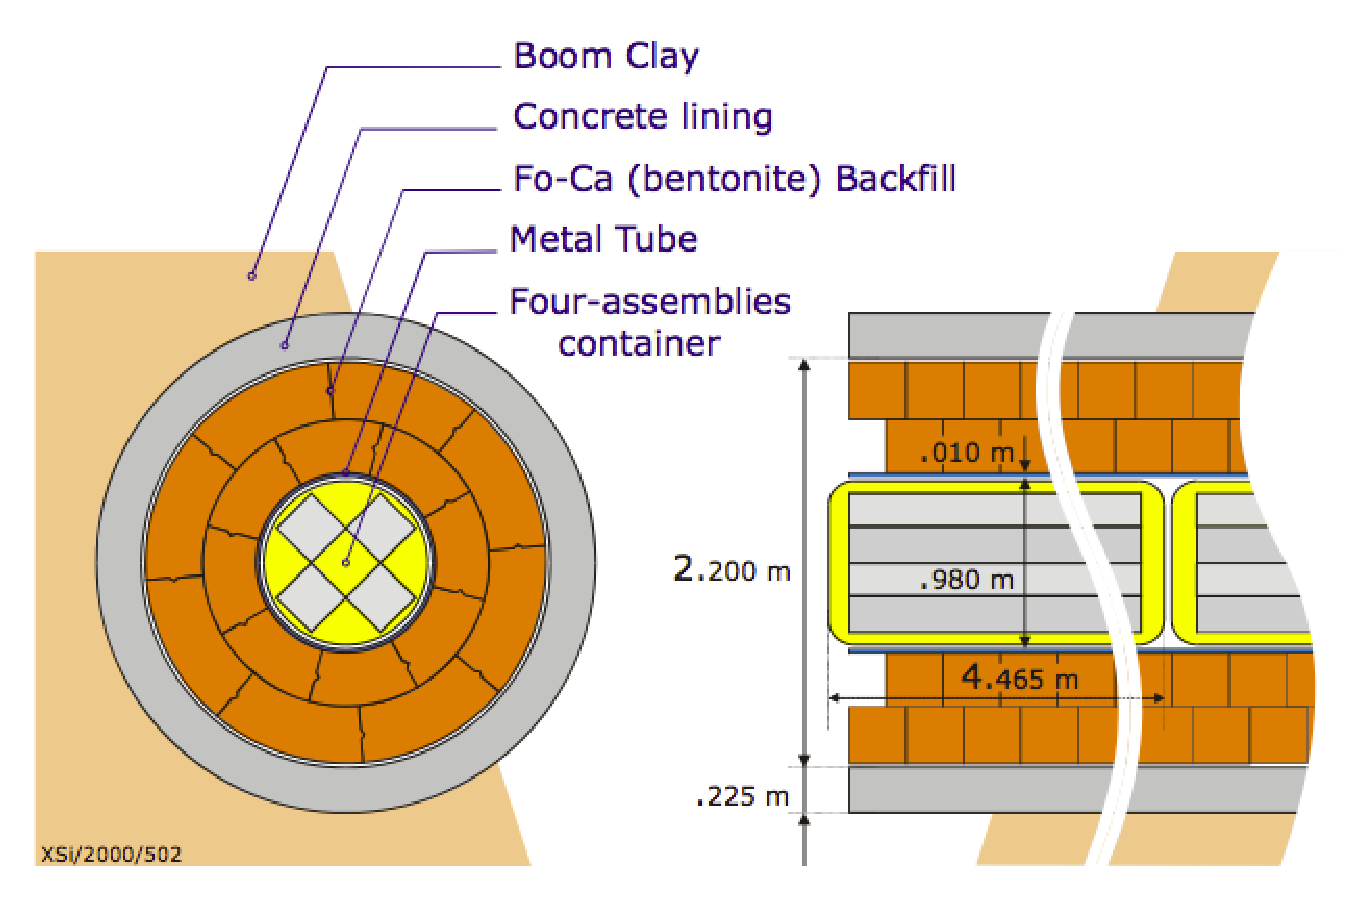
\includegraphics[width=.4\textwidth]{belgianClayRedImp.eps}
         \caption{Belgian reference concept in Boom Clay 
         \cite{von_lensa_red-impact_2008}.}
     \end{figure}
     \begin{figure}[h!]
         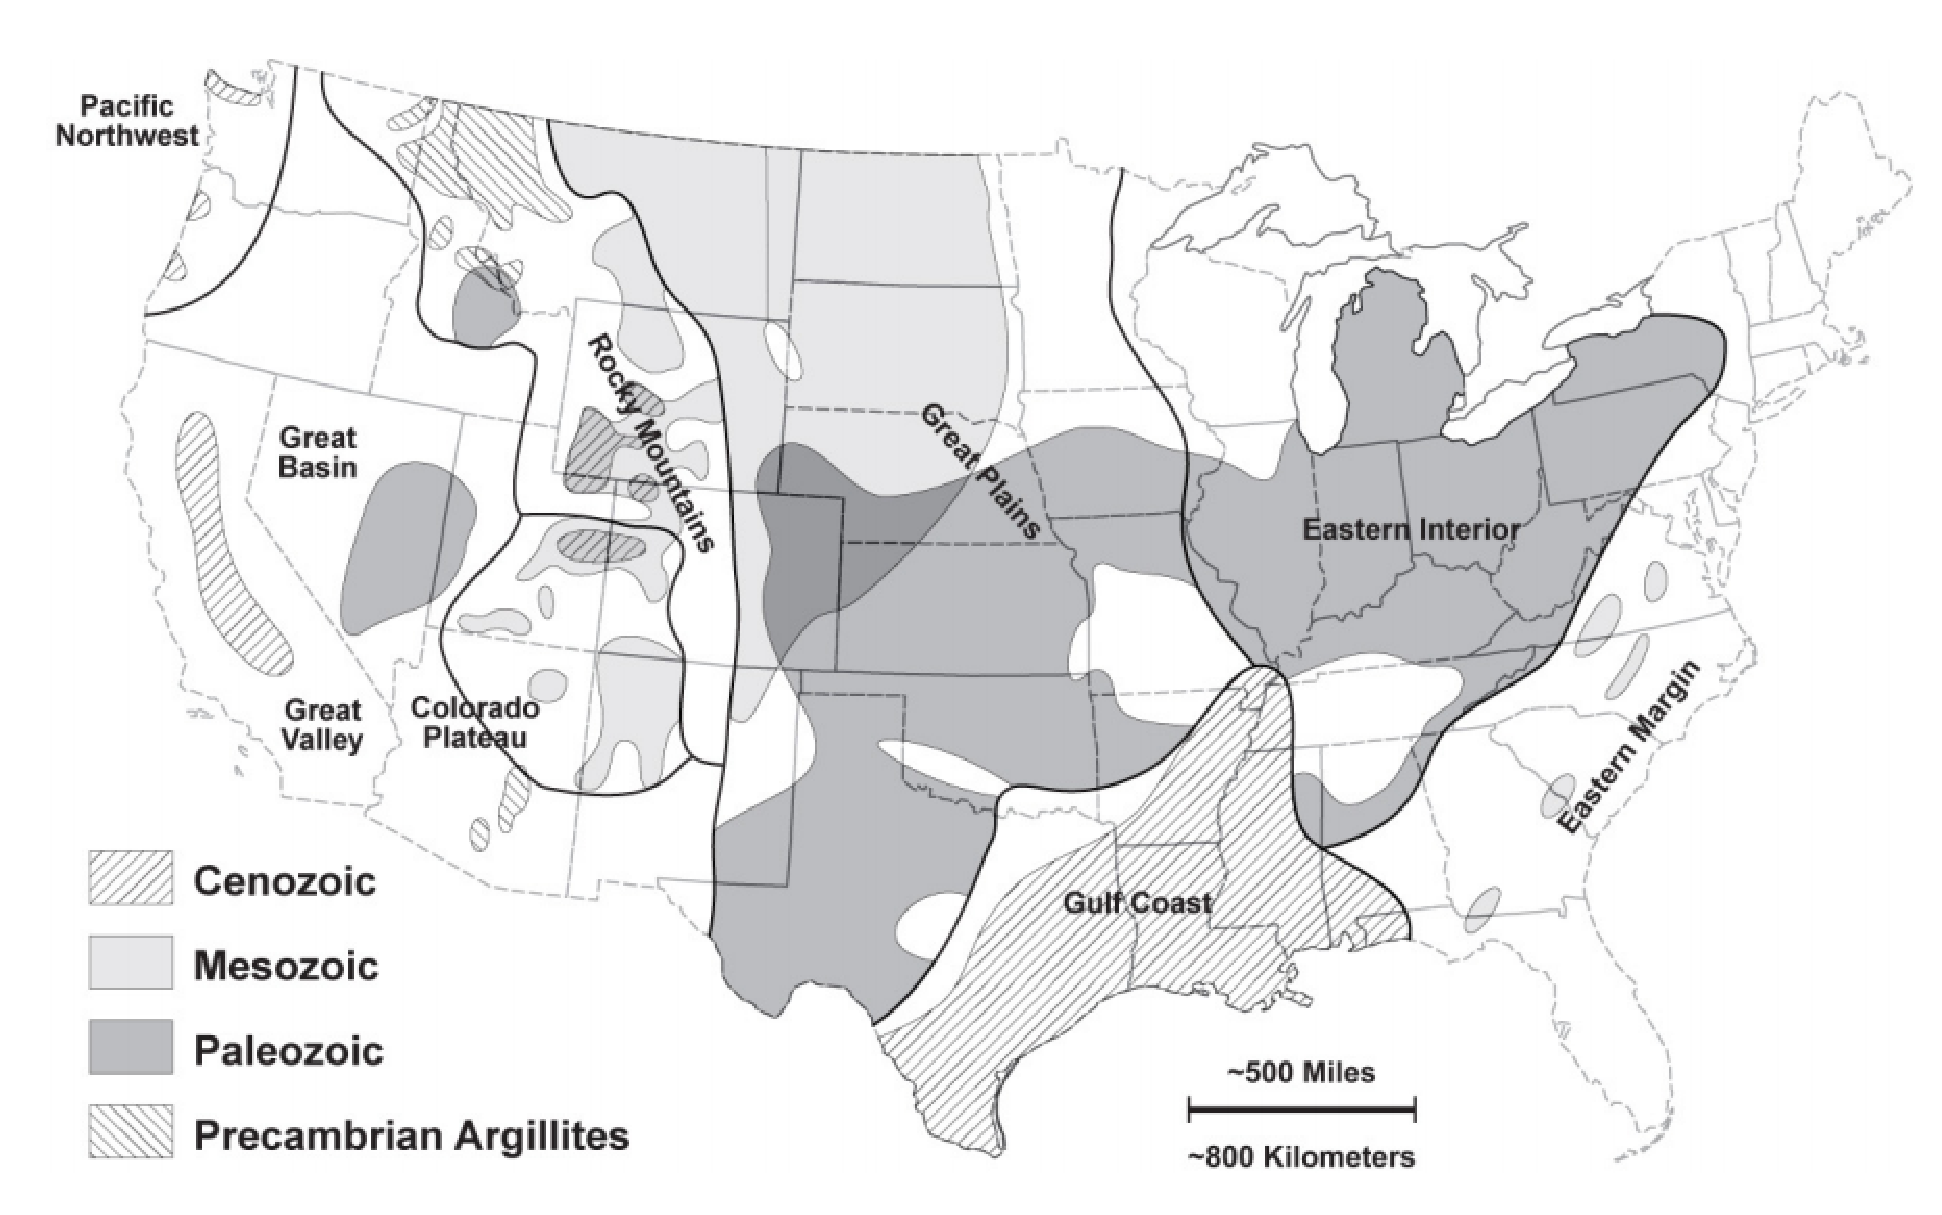
\includegraphics[width=0.4\textwidth]{clayGonzales.eps}
         \caption{U.S. Clay Deposits, ref. \cite{gonzales_shales_1985}.}
     \end{figure}
   \hspace{0.01cm}
\end{frame}



\begin{frame}[c]
  \frametitle{Clay Generic Disposal System Model}
The Clay \gls{GDSM}, developed at Argonne National Lab, is built on the GoldSim 
simulation framework and contaminant transport model.  It simulates chemical and 
physical attenuation processes \cite{golder_goldsim_2010, 
golder_goldsim_ct_2010}, including 
\begin{itemize}
  \item  chemical and physical attenuation processes including
  \item radionuclide solubility,
  \item dispersion phenomena,
  \item and reversible sorption.
\end{itemize}

Input parameters include 
\begin{itemize}
  \item geometry specifications (e.g. repository depth),
  \item geologic material properties (e.g. clay porosity), 
  \item geochemical data (e.g. elemental solubility limits),
  \item and environmental parameters (e.g. natural system velocity). 
\end{itemize}
\end{frame}

\begin{frame}[c]
  \frametitle{Clay Generic Disposal System Model}
  \vspace{2cm}
\begin{figure}[h!]
\includegraphics[width=0.6\textwidth]{feps.eps}
\caption{General Features Events and Processes in the Clay repository model 
  \ref{clayton_generic_2011}.}
\end{figure}
\end{frame}

\begin{frame}[c]
  \frametitle{Clay Generic Disposal System Model}
The disposal concept modeled by the Clay \gls{GDSM} \cite{nutt_generic_2009} is
\begin{itemize}
  \item an array of spent nuclear fuel packages 
  \item emplaced horizontally
  \item in excavated tunnels, 
  \item backfilled by a reducing bentonite clay,
  \item within a clay repository envrionment, 
  \item \textbf{500 meters} beneath the earth's surface.
\end{itemize}
\end{frame}

\begin{frame}[c]
  \frametitle{Mean of the Peak Annual Dose}
In this analysis, repository performance is quantified by radiation dose to a 
hypothetical receptor. Specifically, the mean of the peak annual dose,

\footnotesize{
  \begin{align} \label{MoP}
    D_{MoP,i} &= \frac{\sum_{r=1}^{N}{\max\left[\left.D_{r,i}(t)\right|_{\forall t}\right]}}{N}
    \intertext{where}
    D_{MoP,i} &= \mbox{ mean of peak annual dose due to isotope i } [mrem/yr]\nonumber\\
    D_{r,i}(t) &= \mbox{ year t dose in realization r due to isotope i } [mrem/yr]\nonumber\\
    N &= \mbox{number of realizations, } \nonumber
\end{align}
}

is a conservative metric of repository performance and should not be confused 
with the peak of the mean annual dose.

\footnotesize{
  \begin{align} \label{PoM}
    D_{PoM,i} &= \max\left[{\frac{\sum_{r=1}^{N}{\left.D_{r,i}(t)\right|_{\forall t}}}{N}}\right]\\
              &= \mbox{peak of the mean annual dose due to isotope i } [mrem/yr].\nonumber
  \end{align}
}
\end{frame}

\begin{frame}[c]
  \frametitle{Sampling Strategy}
  \footnotesize{
To develop a many dimensional overview, both individual and dual parametric cases were performed.

\begin{itemize}
  \item \textbf{Individual parameter cases} varied a single parameter of interest in 
detail over a broad range of values. 
  \item \textbf{Dual parameter cases} were performed for pairs of parameters expected to exhibit some covariance. 
\end{itemize}    
For each case, forty simulation 
groups varied the parameter or parameters within the range considered. 
For each simulation group, a 100 realization simulation was completed 
\cite{clayton_generic_2011, 
nutt_generic_2009}.  

\begin{table}[ht!]
\centering
\footnotesize{
\begin{tabular}{|l|l|l|r|r|}
\multicolumn{5}{c}{\textbf{Simulation Cases}}\\
\hline
\textbf{Case} & \textbf{Parameter} & \textbf{Units} & \textbf{Min. Value} & \textbf{Max. Value}\\
\hline
V     & $R_{WFDeg.}$           & $[yr^{-1}]$       & $10^{-9}$    &  $10^{-2}$ \\
      & Inventory              & [MTHM]         & $10^{-4}$    &  $10^1$ \\
\hline
\end{tabular}
\caption{Each dual and single parameter simulation case had 40 simulation 
groups of 100 realizations each.}
\label{tab:Cases}
}
\end{table}


}

\end{frame}


%%%%%%%%%%%%%%%%%%%%%%%%%%%%%%%%%%%%%%%%%%%%%%%%%%%%%%%%%%%%%%%%%%%%%%%%%%%%%%%%
  
\begin{frame}[c]
  \frametitle{Case I : Diffusion Coefficient and Inventory}
The sensitivity of the peak dose to the reference diffusivity of the 
host rock was analyzed.  In this model, the reference diffusivity of the medium 
was the input parameter used to vary the effective diffusivity in a controlled 
manner. In GoldSim's transport module, the effective diffusion coefficient is 
defined as 

\begin{align}\label{diffcoeff}
  D_{eff} &= n\tau D_{ref}D_{rel} \\ % ?  
       D_{eff} &= ~~\mbox{effective diffusion coefficient }[m^2/s],\nonumber\\
       D_{rel} &= ~~\mbox{relative diffusivity for each isotope in water }[\%],\nonumber\\
       D_{ref} &= ~~\mbox{reference diffusivity in water }[m^2/s],\nonumber\\
       \tau &= ~~\mbox{tortuosity} [\%], \nonumber \\ 
       n &= ~~\mbox{porosity}[\%].\nonumber\\
  \label{GDSEdiff}
\end{align}
\end{frame}

\begin{frame}[c]
  \frametitle{Case I : Diffusion Coefficient and Inventory}
The waste inventory total mass was also altered for each value of the reference 
diffusivity.  That is, the radionuclide inventory in a reference 
\gls{MTHM} of commercial spent nuclear fuel was multiplied by a scalar mass factor.  
It was expected that changing these two parameters in tandem would capture the 
importance of diffusivity in the far field to the repository performance 
as well as a threshold at which the effect of waste inventory dissolution is 
attenuated by solubility limits.
\end{frame}

\begin{frame}[c]
  \frametitle{Case I : Diffusion Coefficient and Inventory}
Finally, in order to isolate the effect of the far field behavior, the waste form 
degradation rate was set to be very high as were the solubility and advective 
flow rate through the  \gls{EBS}. This guaranteed that contaminant flowthrough 
in the near field was unhindered, leaving the far field as the dominant barrier 
to release.
\end{frame}

\begin{frame}[c]
  \frametitle{Case I : Diffusion Coefficient and Inventory}
The forty runs corresponded to eight values of relative diffusivity and five 
values of inventory mass multiplier. That is, the reference diffusivity was varied over the 
eight magnitudes between $ 10^{-8}$ and $10^{-15}$ $[m^2 /s]$ . 
The Mass Factor, the unitless inventory multiplier, was simultaneously varied over 
the five magnitudes between $10^{-4}$ and $10^{1} [-]$. That is, the 
radionuclide inventory was varied between $10^{-4}$ and $10^{1}$ of that in one 
\gls{MTHM} of \gls{SNF}, which is expected to cover the full range of 
inventories in current wasteforms.

\begin{frame}[c]
  \frametitle{Case I : Diffusion Coefficient and Inventory}
\begin{table}[hbp!]
\centering
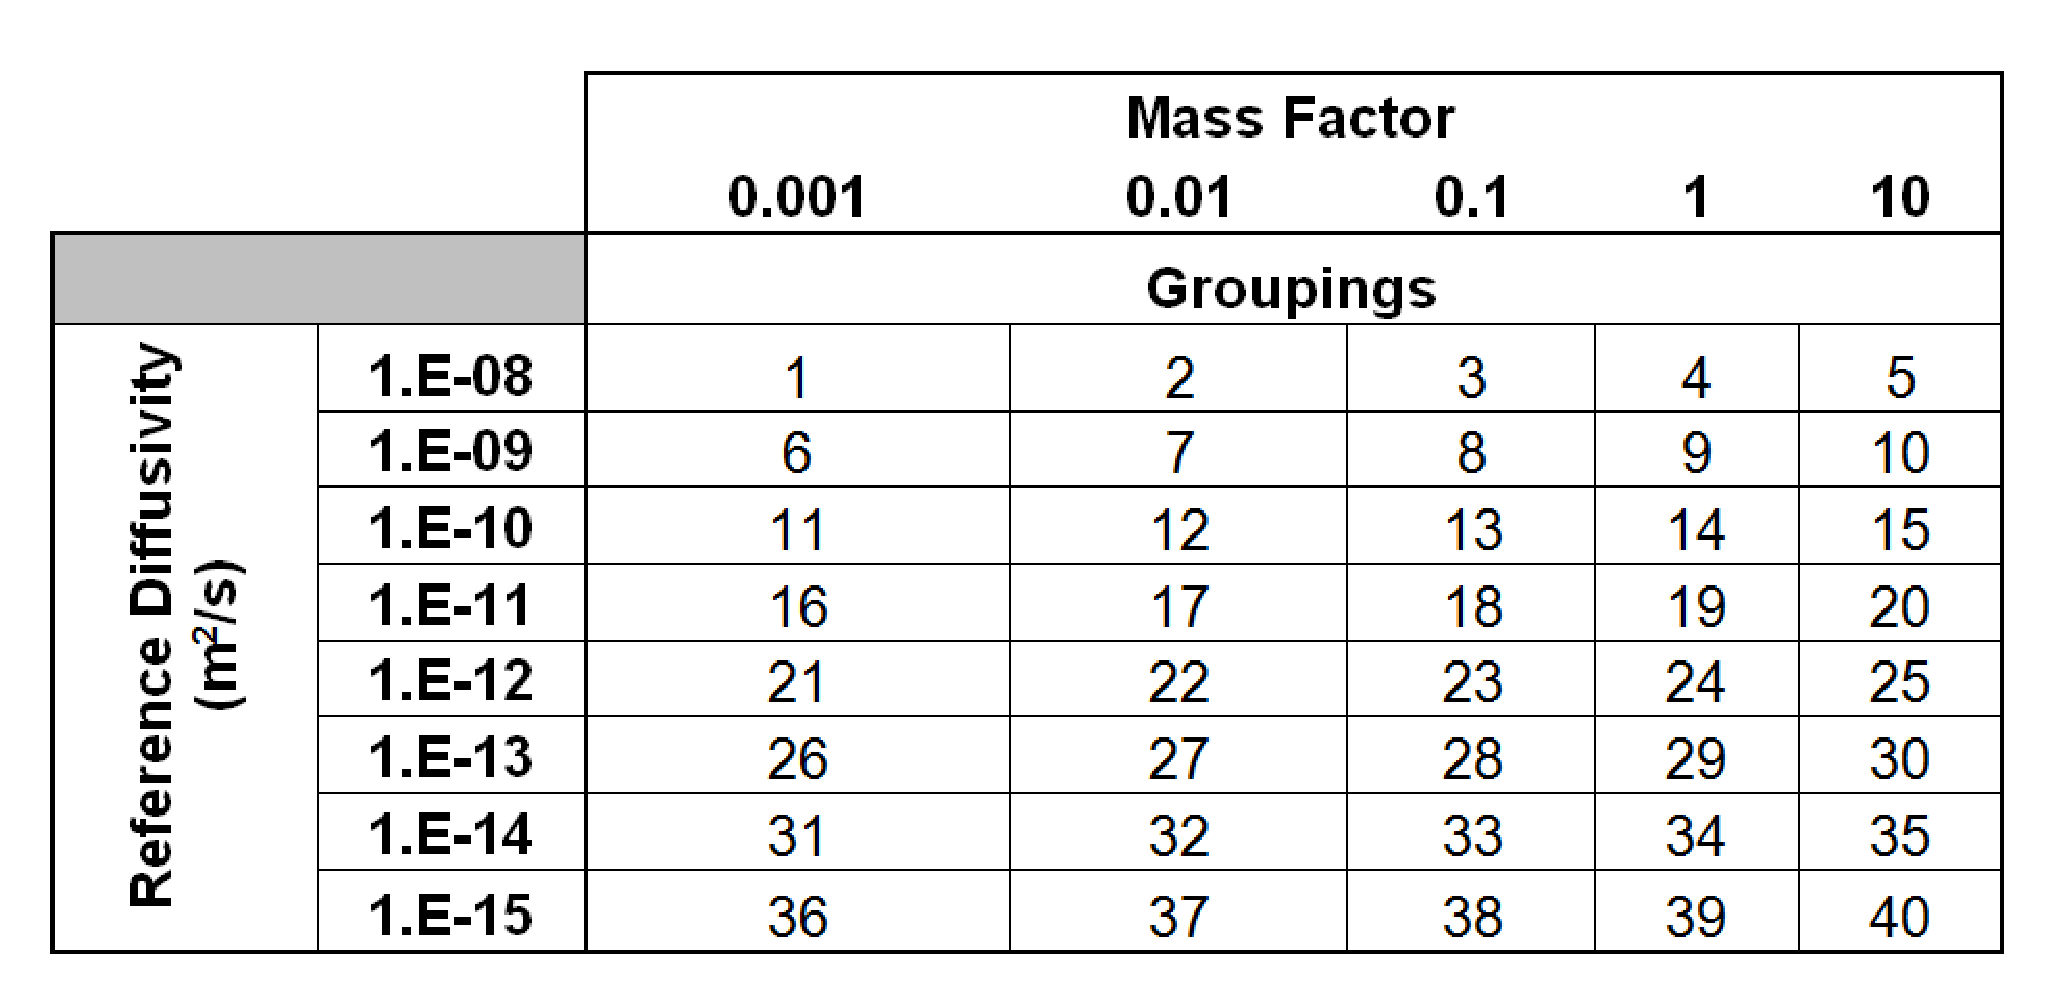
\includegraphics[width=0.7\textwidth]{DiffCoeffAndInvEBSFail/DiffCoeffAndInvGroups.eps}
\caption{Diffusion coefficient and mass factor simulation groupings.}
\label{tab:DiffCoeffAndInvGroups}
\end{table}
\end{frame}

\begin{frame}[c]
  \frametitle{Case I : Diffusion Coefficient and Inventory}
The peak doses due to highly soluble, non-sorbing elements such as $I$ and $Cl$, 
are  proportional to the radionuclide inventory and 
largely directly proportional to the relative diffusivity. This can be seen for 
the cases of $^{129}I$ and $^{36}Cl$ in Figures \ref{fig:DCInvI129}, 
\ref{fig:DCInvI129MF}, \ref{fig:DCInvCl36} and \ref{fig:DCInvCl36MF}.
\end{frame}



\begin{frame}[c]
  \frametitle{Case I : Diffusion Coefficient and Inventory}
\begin{figure}[ht]
\centering
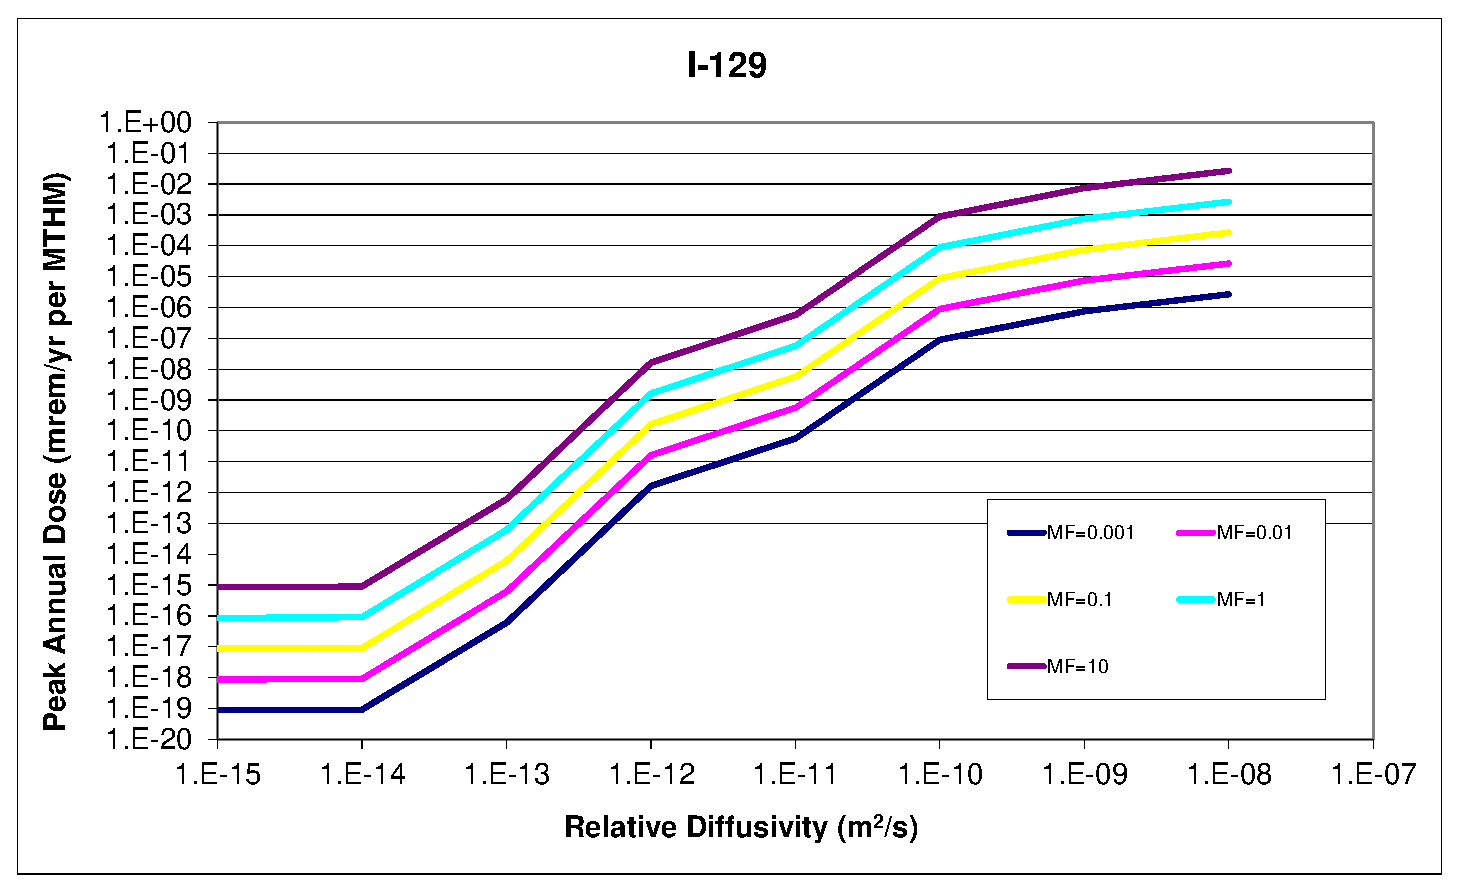
\includegraphics[width=\linewidth]{DiffCoeffAndInvEBSFail/I-129.eps}
\caption{$^{129}I$ relative diffusivity sensitivity.}
\label{fig:DCInvI129}
\end{figure}
\end{frame}

\begin{frame}[c]
  \frametitle{Case I : Diffusion Coefficient and Inventory}
\begin{figure}[ht]
\centering
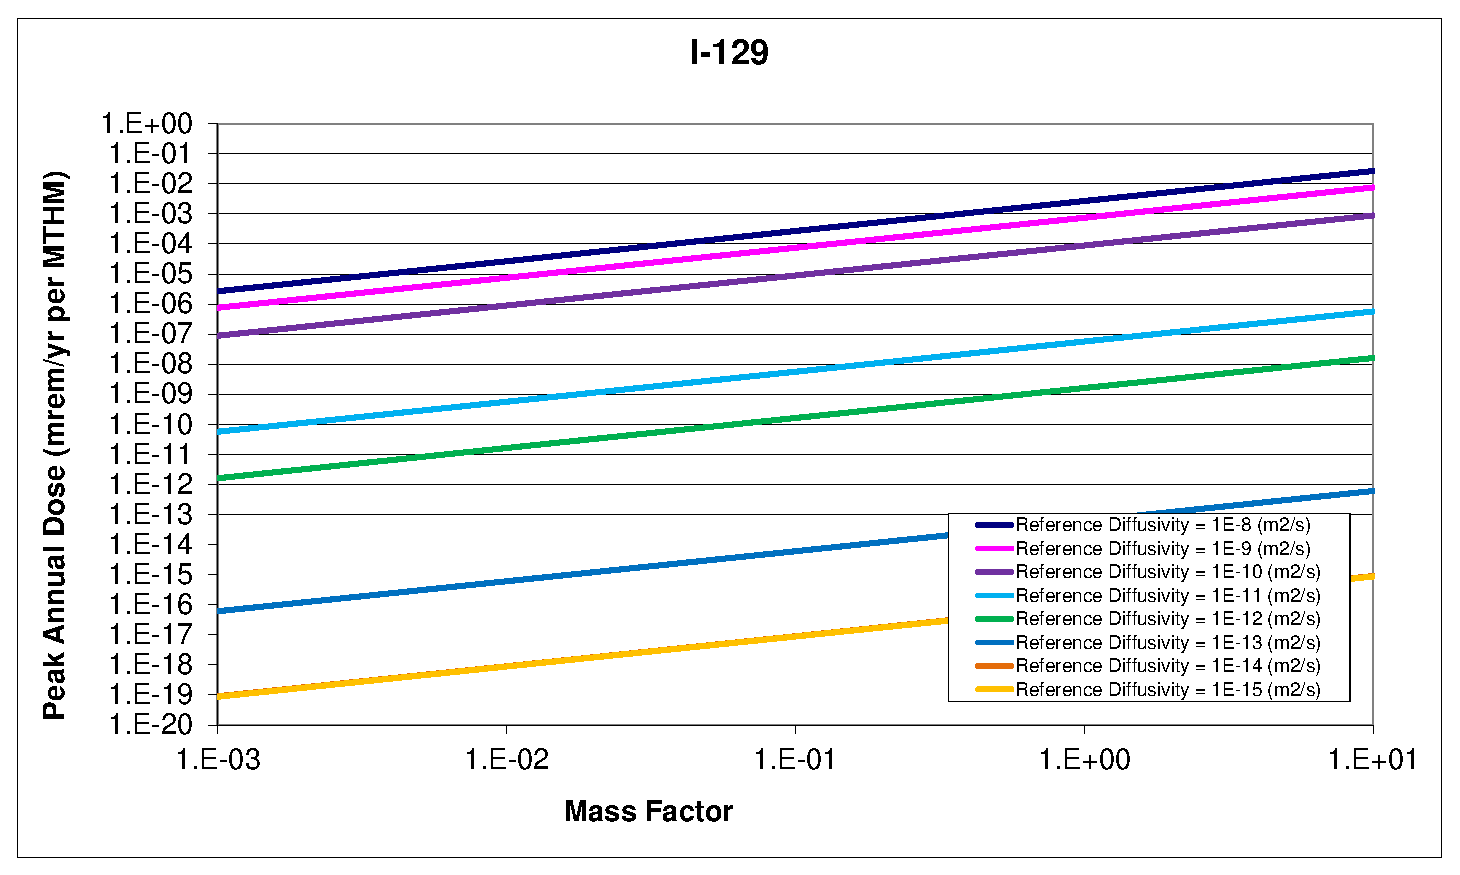
\includegraphics[width=\linewidth]{DiffCoeffAndInvEBSFail/I-129-MF.eps}
\caption{$^{129}I$ mass factor sensitivity.}
\label{fig:DCInvI129MF}
\end{figure}
\end{frame}

\begin{frame}[c]
  \frametitle{Case I : Diffusion Coefficient and Inventory}

\begin{figure}[ht]
\centering
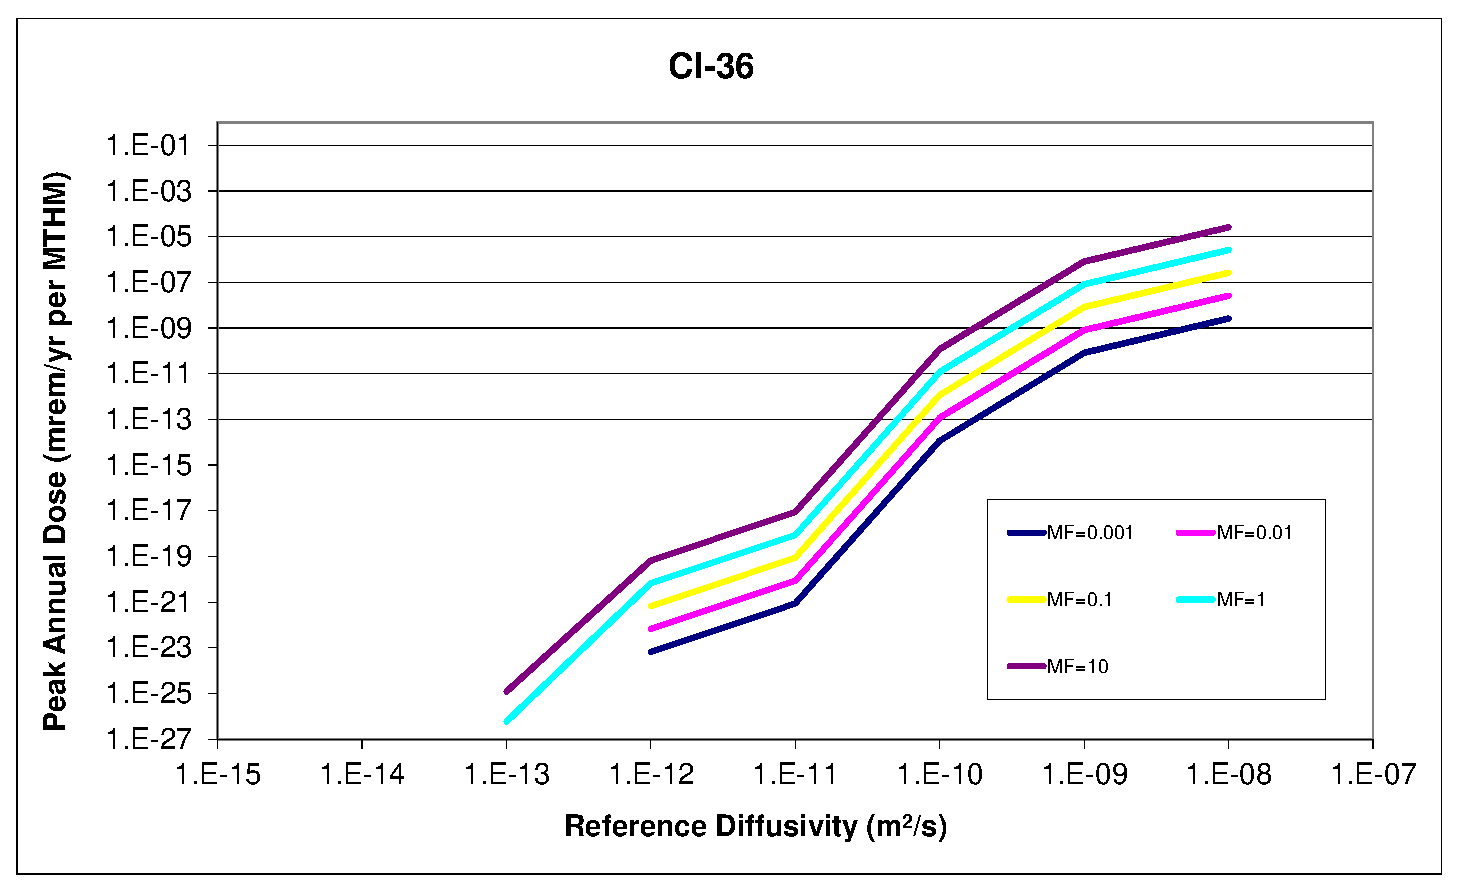
\includegraphics[width=\linewidth]{DiffCoeffAndInvEBSFail/Cl-36.eps}
\caption{$^{36}Cl$ relative diffusivity sensitivity.}
\label{fig:DCInvCl36}
\end{figure}
\end{frame}

\begin{frame}[c]
  \frametitle{Case I : Diffusion Coefficient and Inventory}

\begin{figure}[ht]
\centering
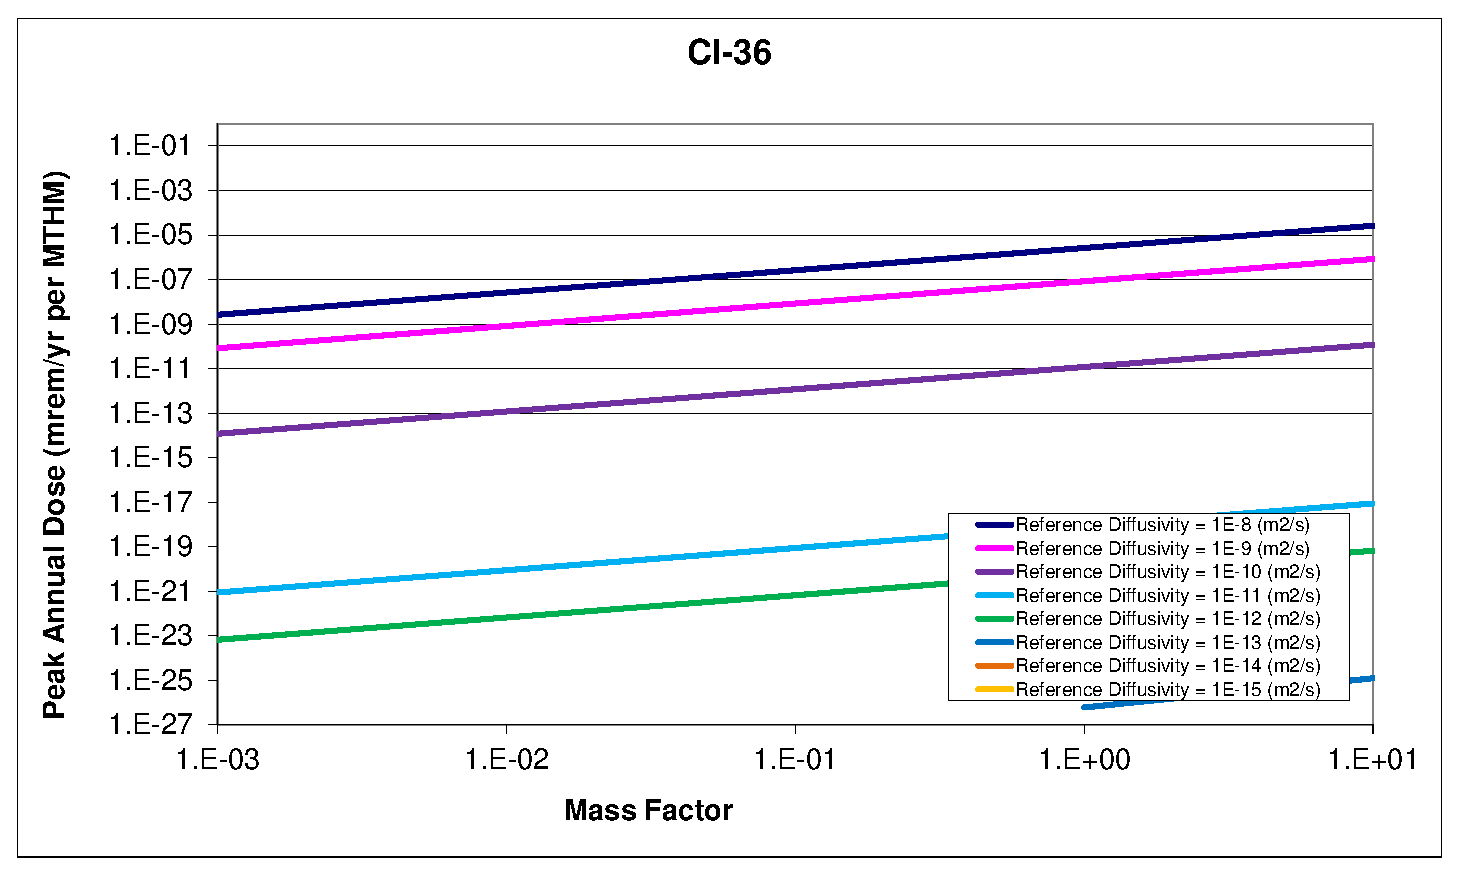
\includegraphics[width=\linewidth]{DiffCoeffAndInvEBSFail/Cl-36-MF.eps}
\caption{$^{36}Cl$ mass factor sensitivity.}
\label{fig:DCInvCl36MF}
\end{figure}
\end{frame}


\begin{frame}[c]
  \frametitle{Case I : Diffusion Coefficient and Inventory}

\begin{figure}[ht!]
\centering
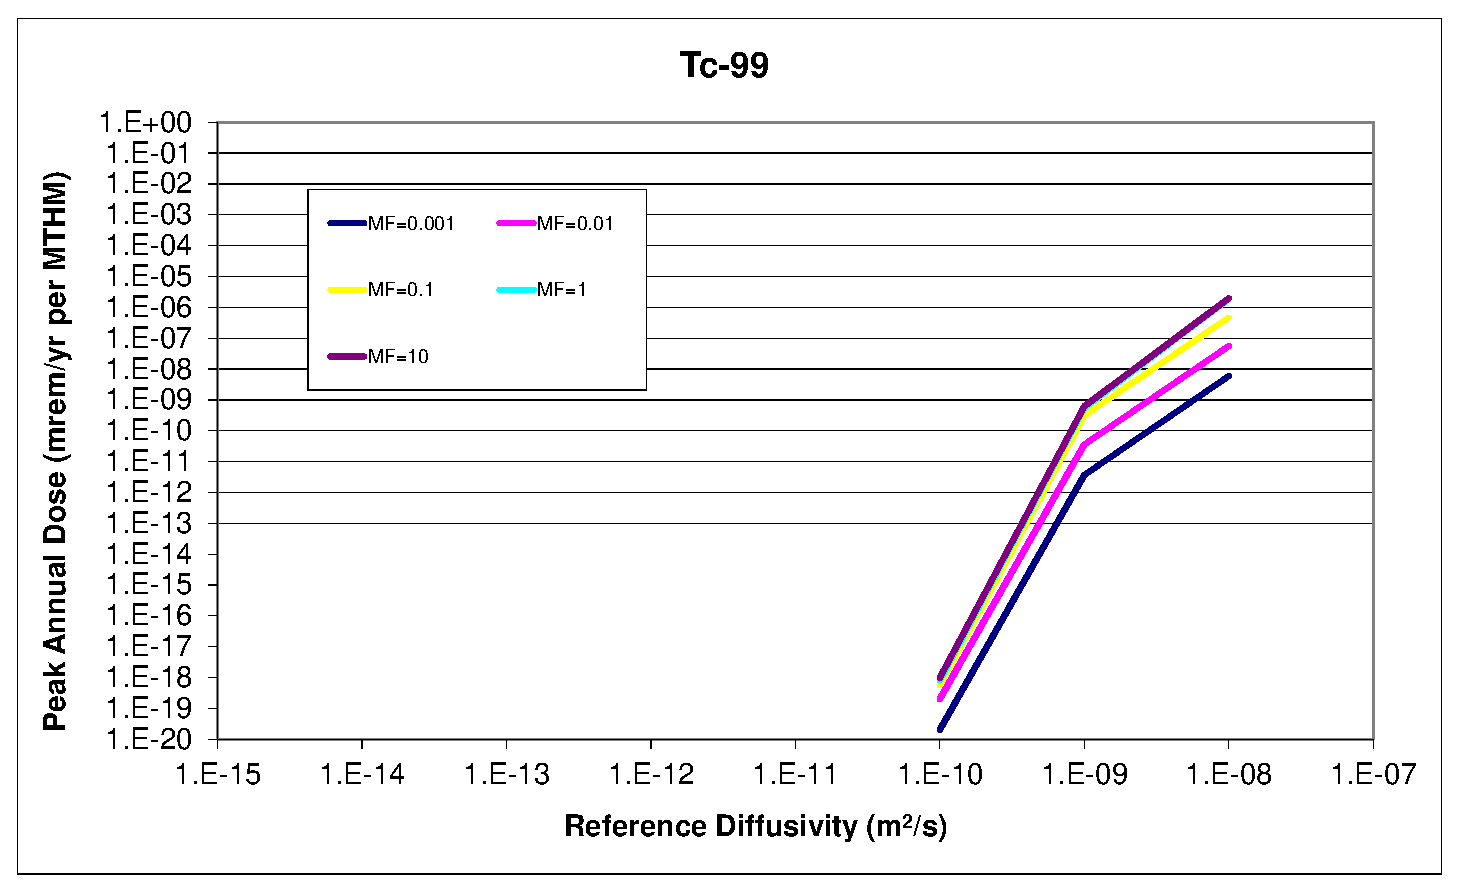
\includegraphics[width=\linewidth]{DiffCoeffAndInvEBSFail/Tc-99.eps}
\caption{$^{99}Tc$ relative diffusivity sensitivity.} 
\label{fig:DCInvTc99}
\end{figure}
\end{frame}

\begin{frame}[c]
  \frametitle{Case I : Diffusion Coefficient and Inventory}

\begin{figure}[ht!]
\centering
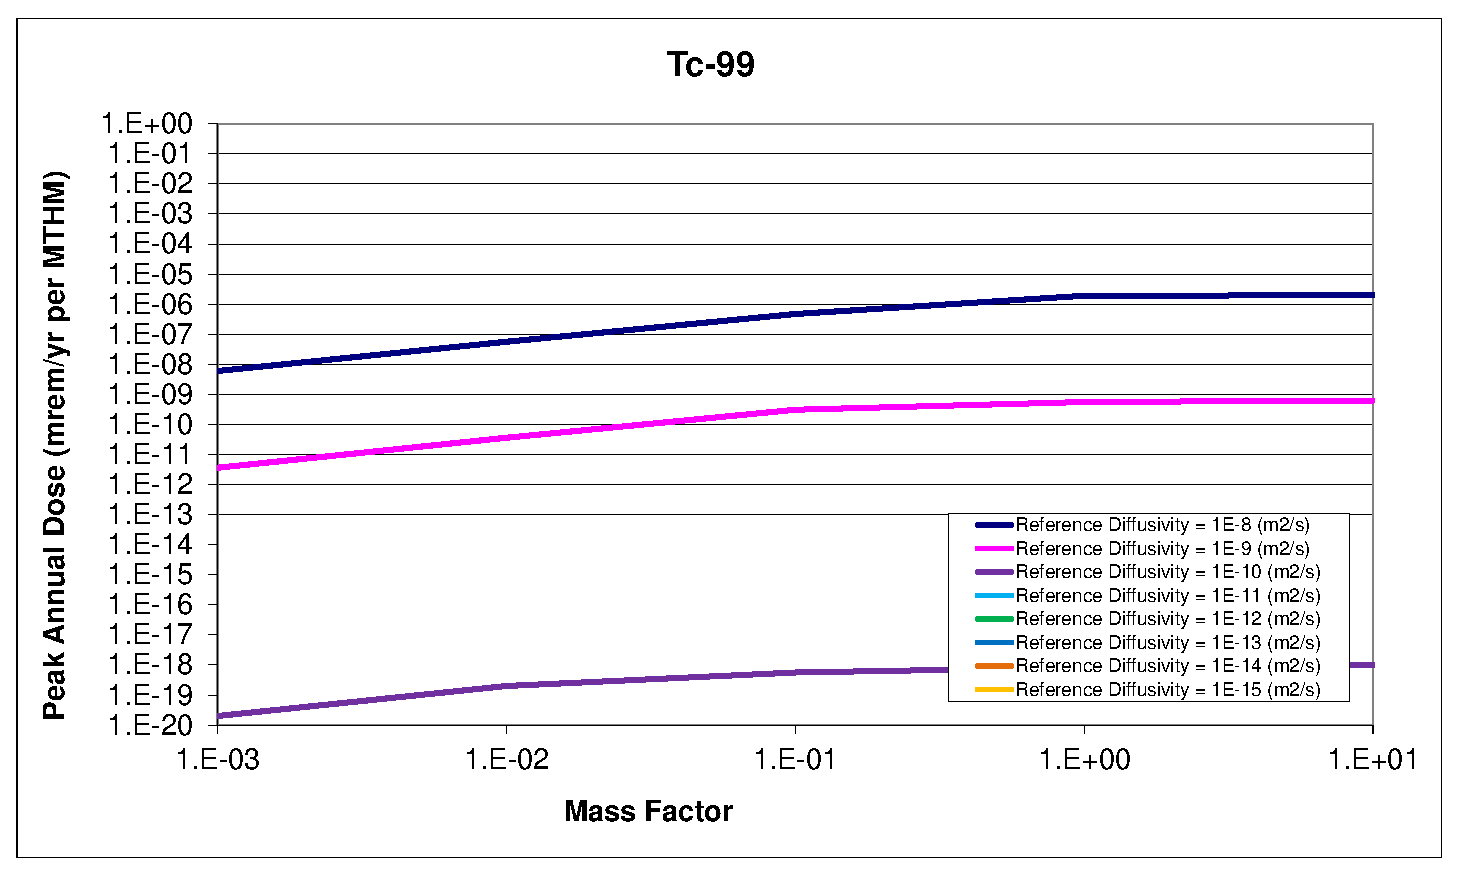
\includegraphics[width=\linewidth]{DiffCoeffAndInvEBSFail/Tc-99-MF.eps}
\caption{$^{99}Tc$ mass factor sensitivity.}
\label{fig:DCInvTc99MF}
\end{figure}
\end{frame}

\begin{frame}[c]
  \frametitle{Case I : Diffusion Coefficient and Inventory}


\begin{figure}[ht!]
\centering
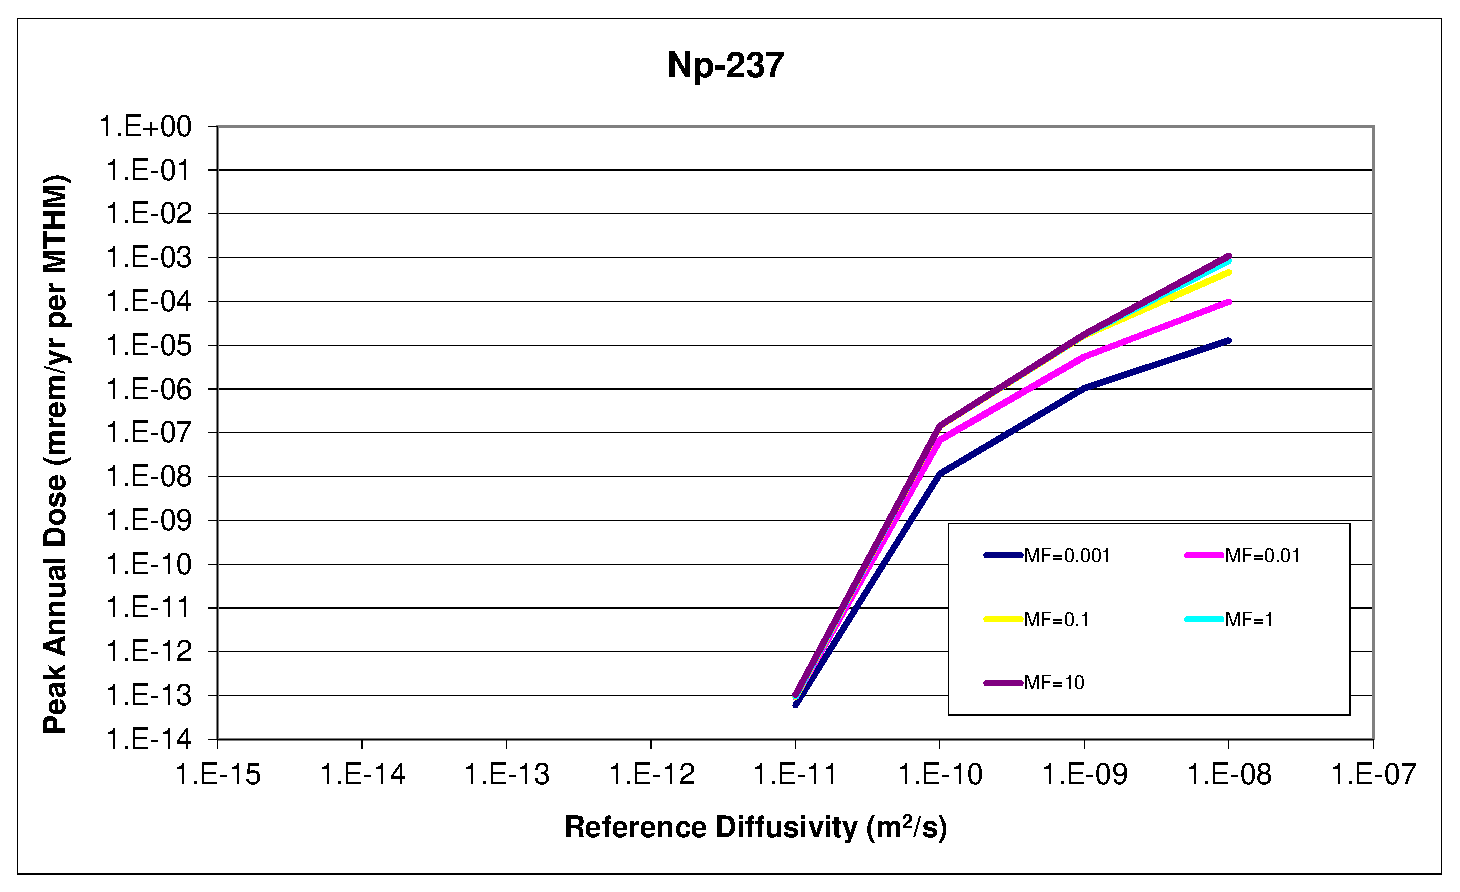
\includegraphics[width=\linewidth]{DiffCoeffAndInvEBSFail/Np-237.eps}
\caption{$^{237}Np$ relative diffusivity sensitivity.} 
\label{fig:DCInvNp237}
\end{figure}
\end{frame}

\begin{frame}[c]
  \frametitle{Case I : Diffusion Coefficient and Inventory}

\begin{figure}[ht!]
\centering
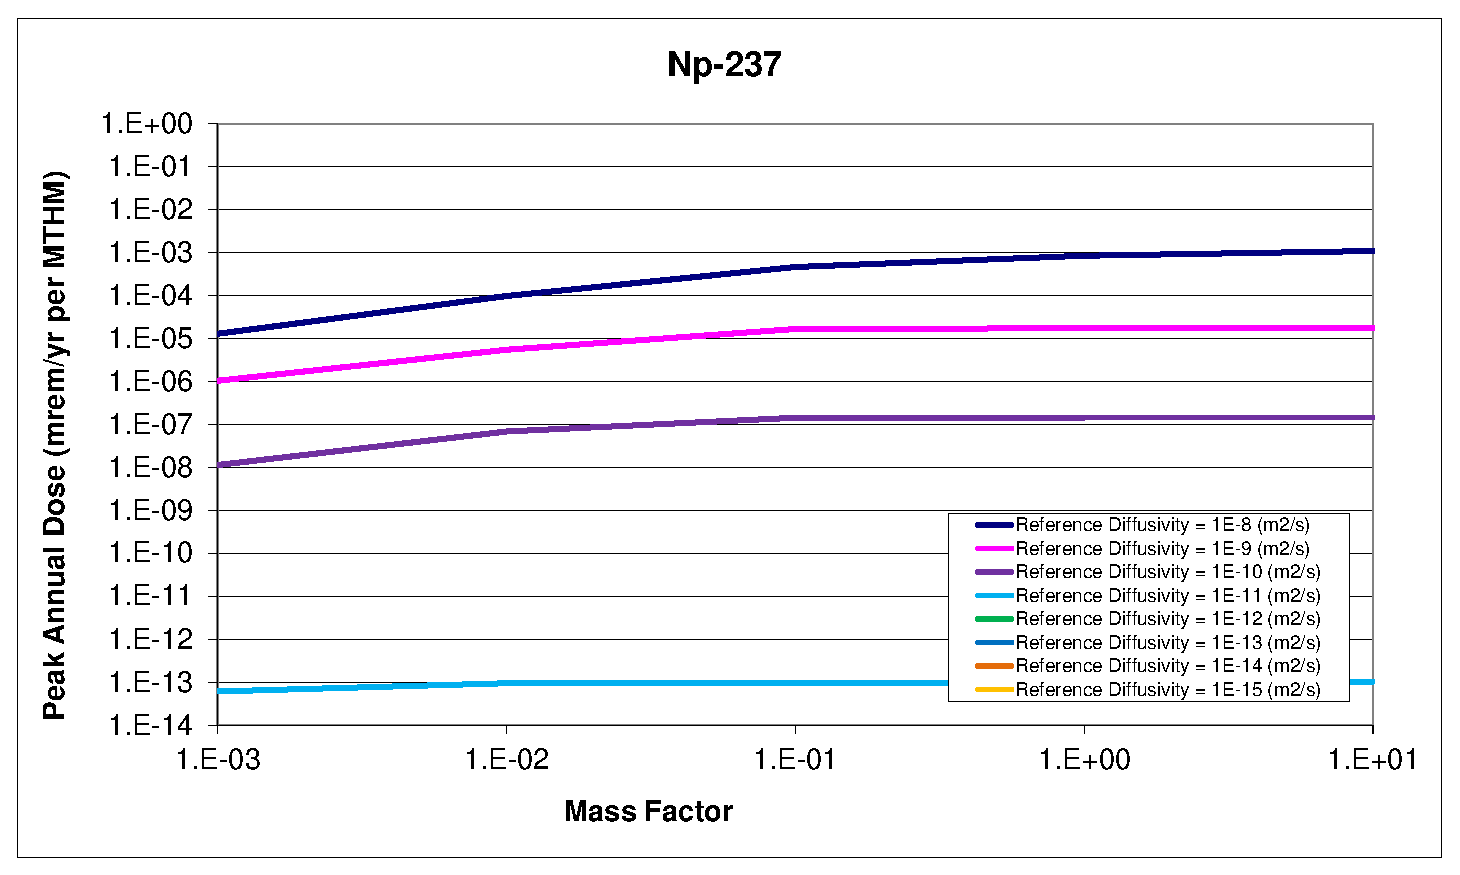
\includegraphics[width=\linewidth]{DiffCoeffAndInvEBSFail/Np-237-MF.eps}
\caption{$^{237}Np$ mass factor sensitivity.}
\label{fig:DCInvNp237MF}
\end{figure}
\end{frame}

\begin{frame}[c]
  \frametitle{Case II : Vertical Advective Velocity and Diffusion Coefficient}
Advection is transport driven by bulk water velocity while diffusion is the 
result of Brownian motion across concentration gradients.  The method by which 
the dominant solute transport mode (diffusive or advective) is determined for a 
particular porous medium is by use of the dimensionless Peclet number, 

\begin{align} 
  Pe &= \frac{nvL}{\alpha nv + D_{eff}},\\
  &= \frac{\mbox{advective rate}}{\mbox{diffusive rate}}\nonumber
  \intertext{where} 
  n &= \mbox{ solute accessible porosity } [\%]\nonumber\\
  v &= \mbox{ advective velocity } [m\cdot s^{-1}] \nonumber\\
  L &= \mbox{ transport distance } [m]\nonumber\\
  \alpha &= \mbox{ dispersivity } [m]\nonumber\\
  D_{eff} &= \mbox{ effective diffusion coefficient } [m^2\cdot s^{-1}].\nonumber
\end{align}
For a high $Pe$ number, advection is the dominant transport mode, while 
diffusive or dispersive transport dominates for a low $Pe$ number
\cite{schwartz_fundamentals_2004}.
\end{frame}

\begin{frame}[c]
  \frametitle{Case II : Vertical Advective Velocity and Diffusion Coefficient}
  \begin{table}[ht!]
\centering
\footnotesize{
\begin{tabular}{|l|l|l|r|r|}
\multicolumn{5}{c}{\textbf{Simulation Cases}}\\
\hline
\textbf{Case} & \textbf{Parameter} & \textbf{Units} & \textbf{Min. Value} & \textbf{Max. Value}\\
\hline
II    & $V_{adv, y}$ & $[m \cdot yr^{-1}]$       & $6.31\times10^{-8}$  &  $6.31\times10^{-4}$ \\
      & $D_{eff}$    & $[m^2\cdot s^{-1}]$       & $10^{-8}$    &  $10^{-5}$ \\
\hline
\end{tabular}
\caption{Case II varied the advective velocity and effective diffusivity to 
  determine the nature of the threshold between the diffusive and advective 
  regimes. This dual parameter simulation case had 40 simulation 
groups of 100 realizations each.}
\label{tab:Cases}
}
\end{table}



The forty runs are a combination of the five values of the vertical advective 
velocity and eight magnitudes of relative diffusivity.
\begin{table}
\centering
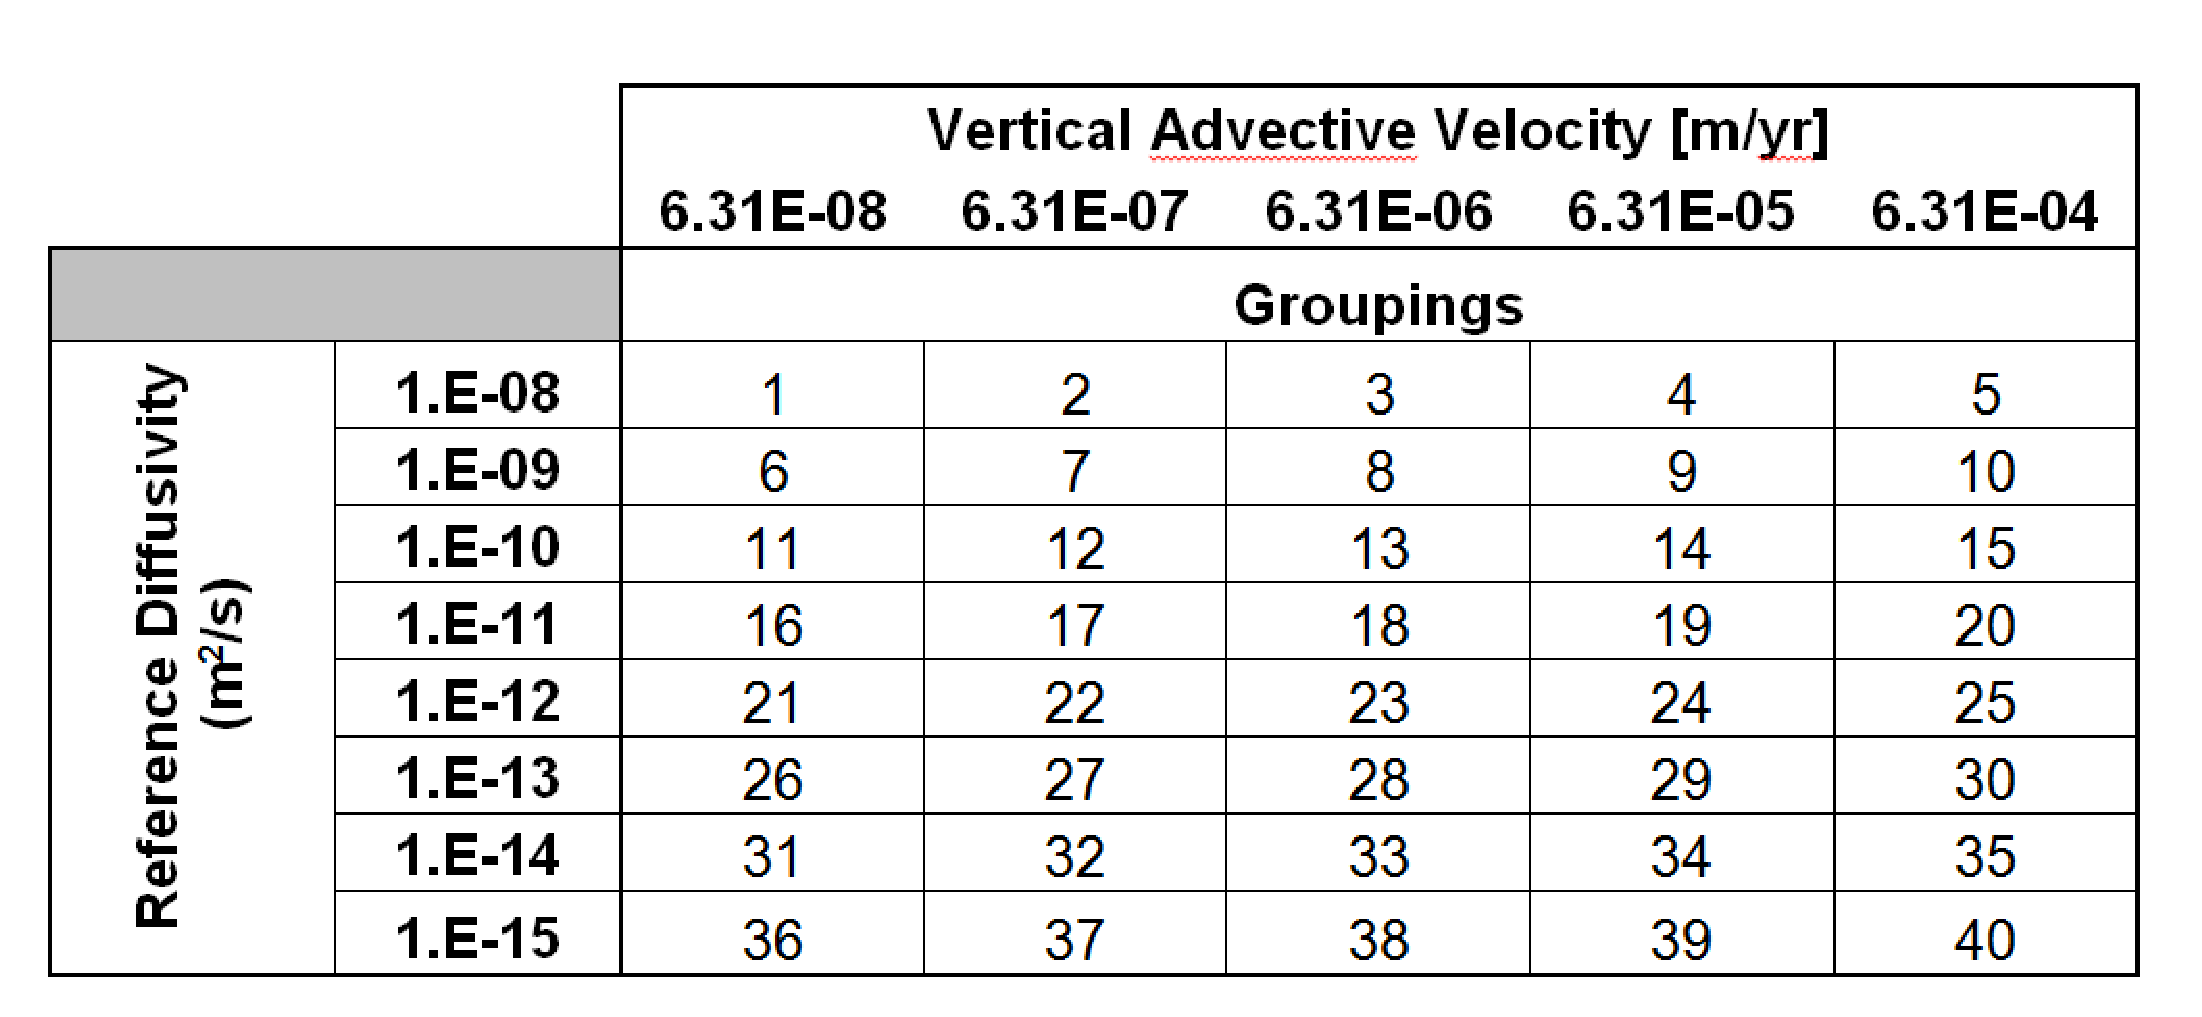
\includegraphics[width=0.8\textwidth]{AdvVelAndDiffCoeffEBSFail/AdvVelAndDiffCoeffGroups.eps}
\caption{Vertical advective velocity and diffusion coefficient simulation groupings.}
\label{tab:AdvVelAndDiffCoeffGroups}
\end{table}
\end{frame}

\begin{frame}[c]
  \frametitle{Case II : Vertical Advective Velocity and Diffusion Coefficient}
\begin{figure}[htp!]
\centering
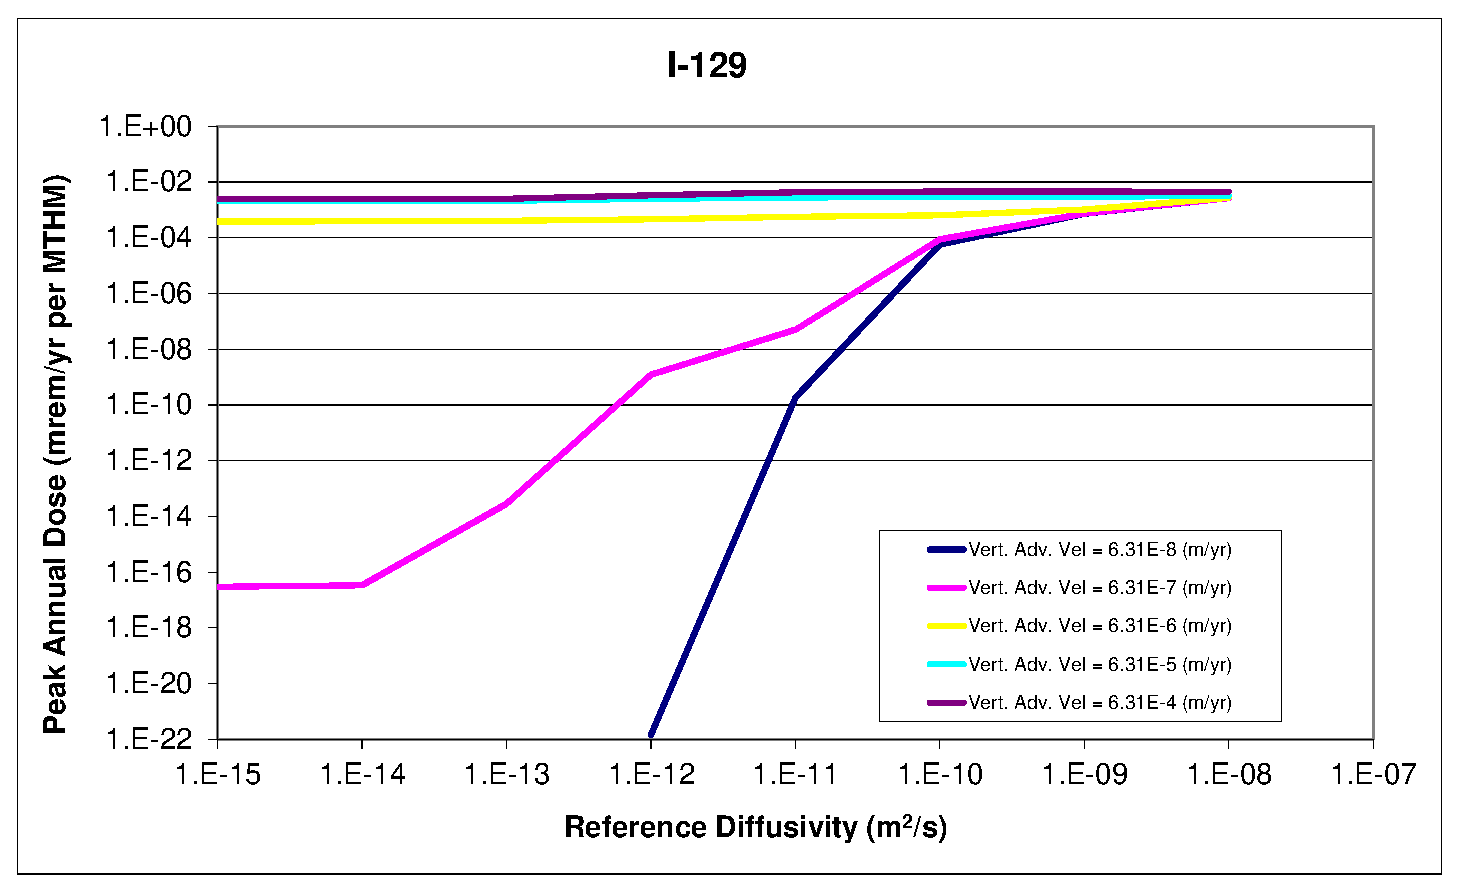
\includegraphics[width=0.8\textwidth]{AdvVelAndDiffCoeffEBSFail/I-129.eps}
\caption{$^{129}I$. For vertical advective velocities 
$6.31\times10^{-6}[m/yr]$ and above, lower reference diffusivities are 
ineffective at attenuating the mean of the peak doses for soluble, non-sorbing 
elements. 
}
\label{fig:VAdvVelI129}
\end{figure}
\end{frame}

\begin{frame}[c]
  \frametitle{Case II : Vertical Advective Velocity and Diffusion Coefficient}
\begin{figure}[htp!]
\centering
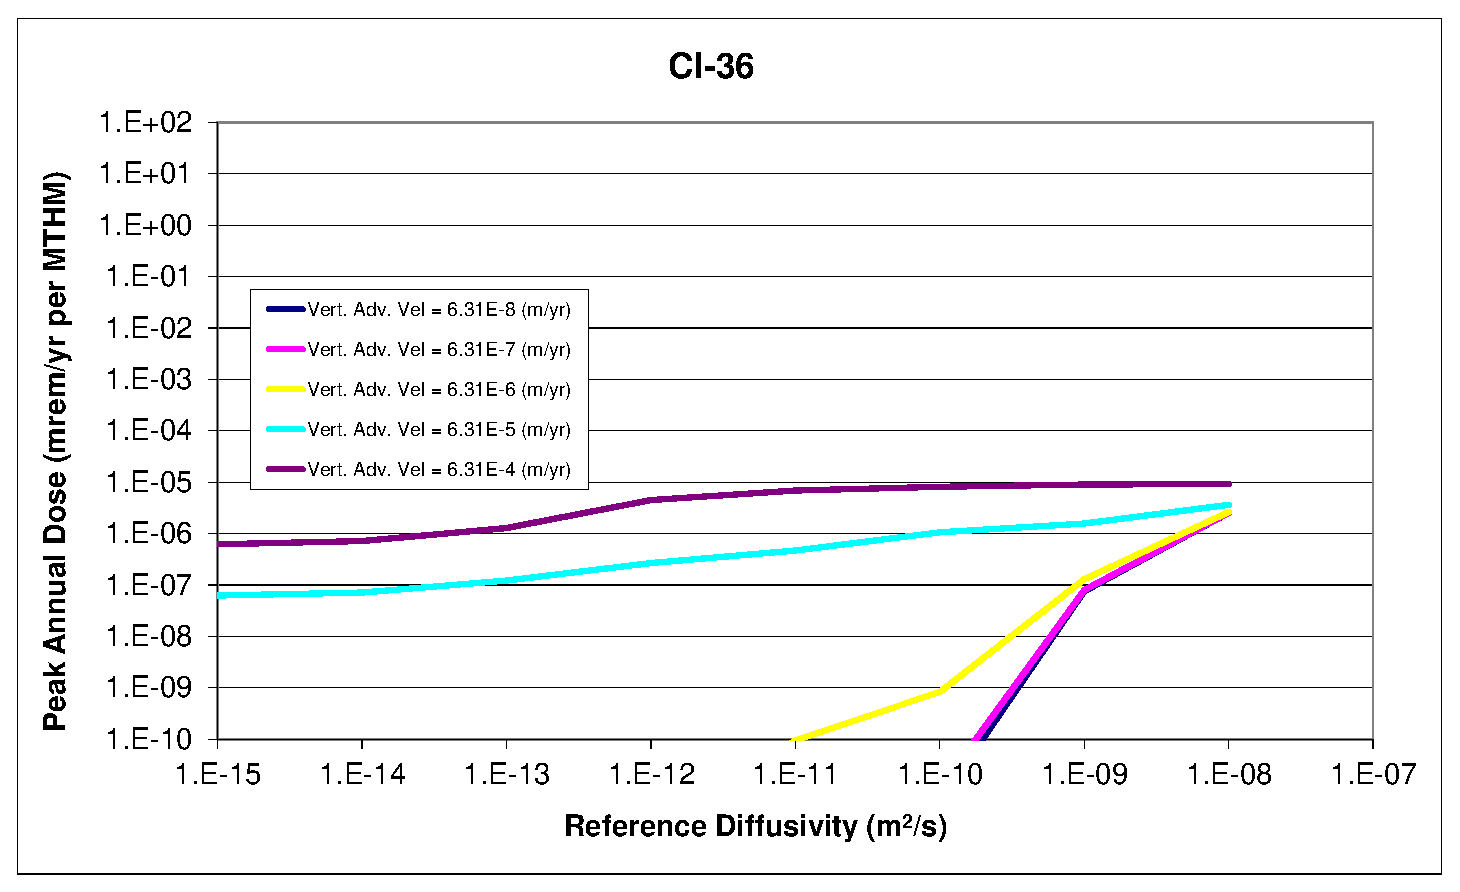
\includegraphics[width=0.8\textwidth]{AdvVelAndDiffCoeffEBSFail/Cl-36.eps}
\caption{$^{36}Cl$.
For vertical advective velocities 
$6.31\times10^{-6}[m/yr]$ and above, lower reference diffusivities are 
ineffective at attenuating the mean of the peak doses for soluble, non-sorbing 
elements. 
}
\label{fig:VAdvVelCl36}
\end{figure}
\end{frame}


\begin{frame}[c]
  \frametitle{Case II : Vertical Advective Velocity and Diffusion Coefficient}

\begin{figure}[ht!]
\centering
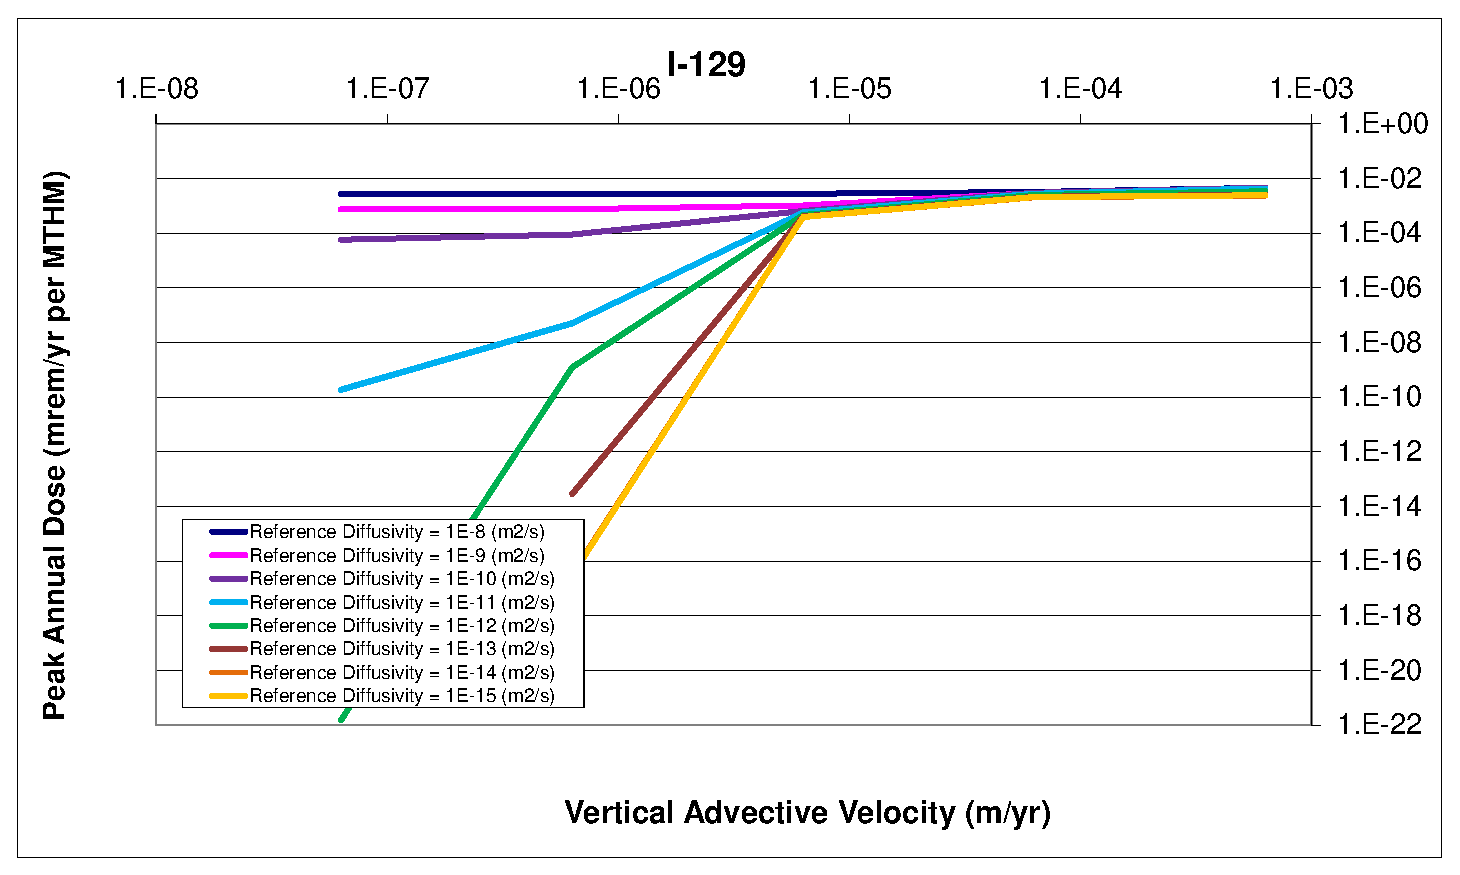
\includegraphics[width=0.8\textwidth]{AdvVelAndDiffCoeffEBSFail/I-129-VAdvVel.eps}
\caption{$^{129}I$.
For vertical advective velocities 
$6.31\times10^{-6}[m/yr]$ and above, lower reference diffusivities are 
ineffective at attenuating the mean of the peak doses for soluble, non-sorbing 
elements. 
}
\label{fig:VAdvVelI129VAdvVel}
\end{figure}
\end{frame}



\begin{frame}[c]
  \frametitle{Case II : Vertical Advective Velocity and Diffusion Coefficient}
\begin{figure}[ht!]
\centering
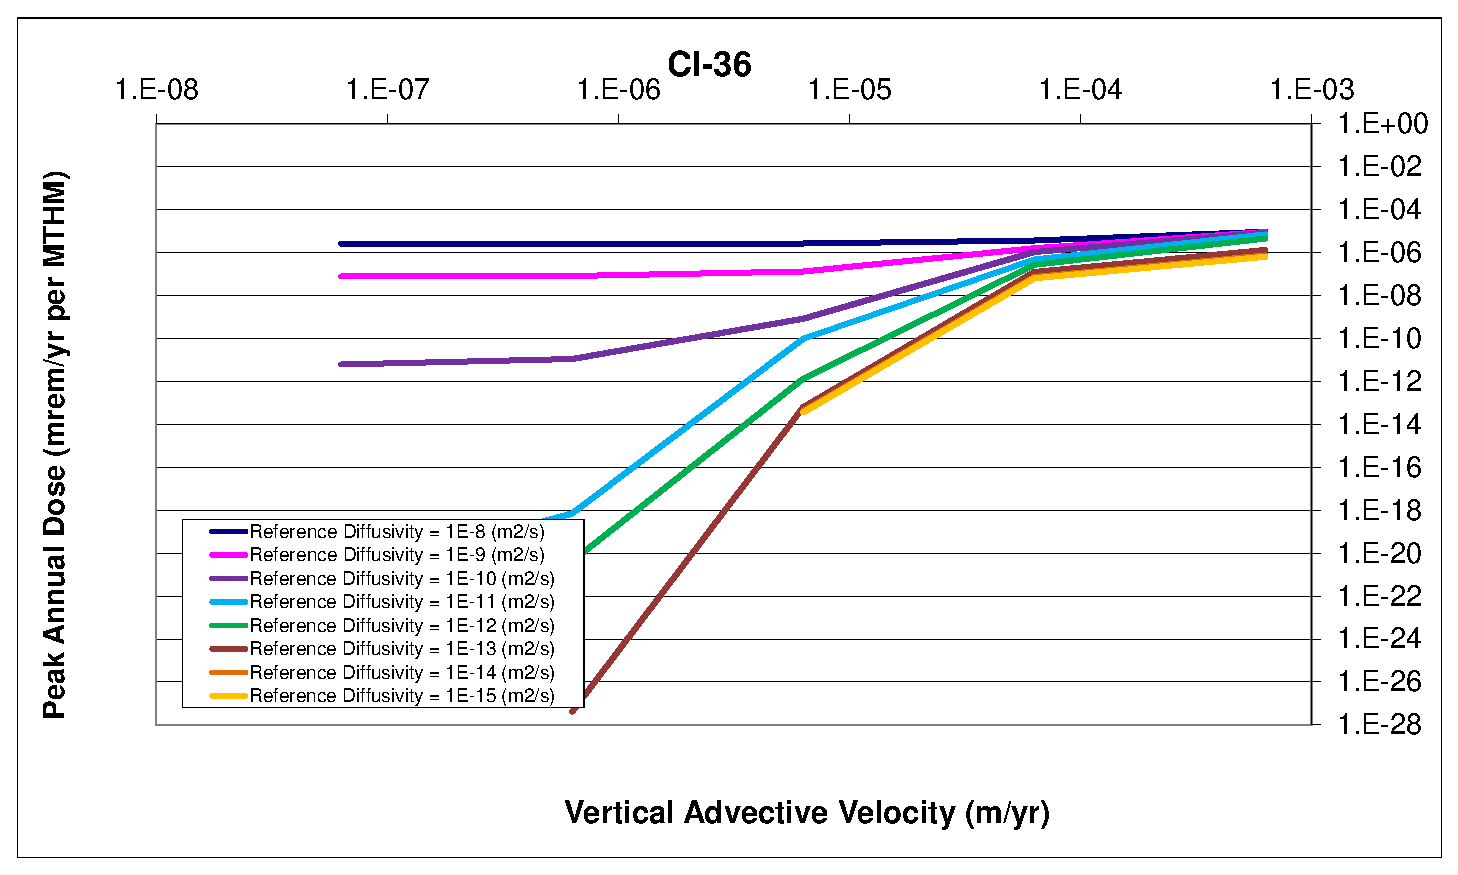
\includegraphics[width=0.8\textwidth]{AdvVelAndDiffCoeffEBSFail/Cl-36-VAdvVel.eps}
\caption{$^{36}Cl$.
For vertical advective velocities 
$6.31\times10^{-6}[m/yr]$ and above, lower reference diffusivities are 
ineffective at attenuating the mean of the peak doses for soluble, non-sorbing 
elements. 
}
\label{fig:VAdvVelCl36VAdvVel}
\end{figure}
\end{frame}

\begin{frame}[c]
  \frametitle{Case II : Vertical Advective Velocity and Diffusion Coefficient}
The solubility limited and sorbing elements, $Tc$ and $Np$, in Figures 
\ref{fig:VAdvVelTc99}, \ref{fig:VAdvVelTc99VAdvVel}, \ref{fig:VAdvVelNp237}, and 
\ref{fig:VAdvVelNp237VAdvVel}

Dose contribution from $^{99}Tc$ has a proportional 
relationship with vertical advective velocity above a regime threshold at 
$6.31\times10^{-5}[m/yr]$, above which the system exhibits sensitivity to 
advection. 

%There is an interesting feature in which $^{99}Tc$ 
%exhibits a decrease in peak annual dose for an increase in reference diffusivity 
%for the very high ($6.31\times10^{-4}$) vertcial advective velocity case. %WHY? 
\end{frame}

\begin{frame}[c]
  \frametitle{Case II : Vertical Advective Velocity and Diffusion Coefficient}
\begin{figure}[htp!]
\centering
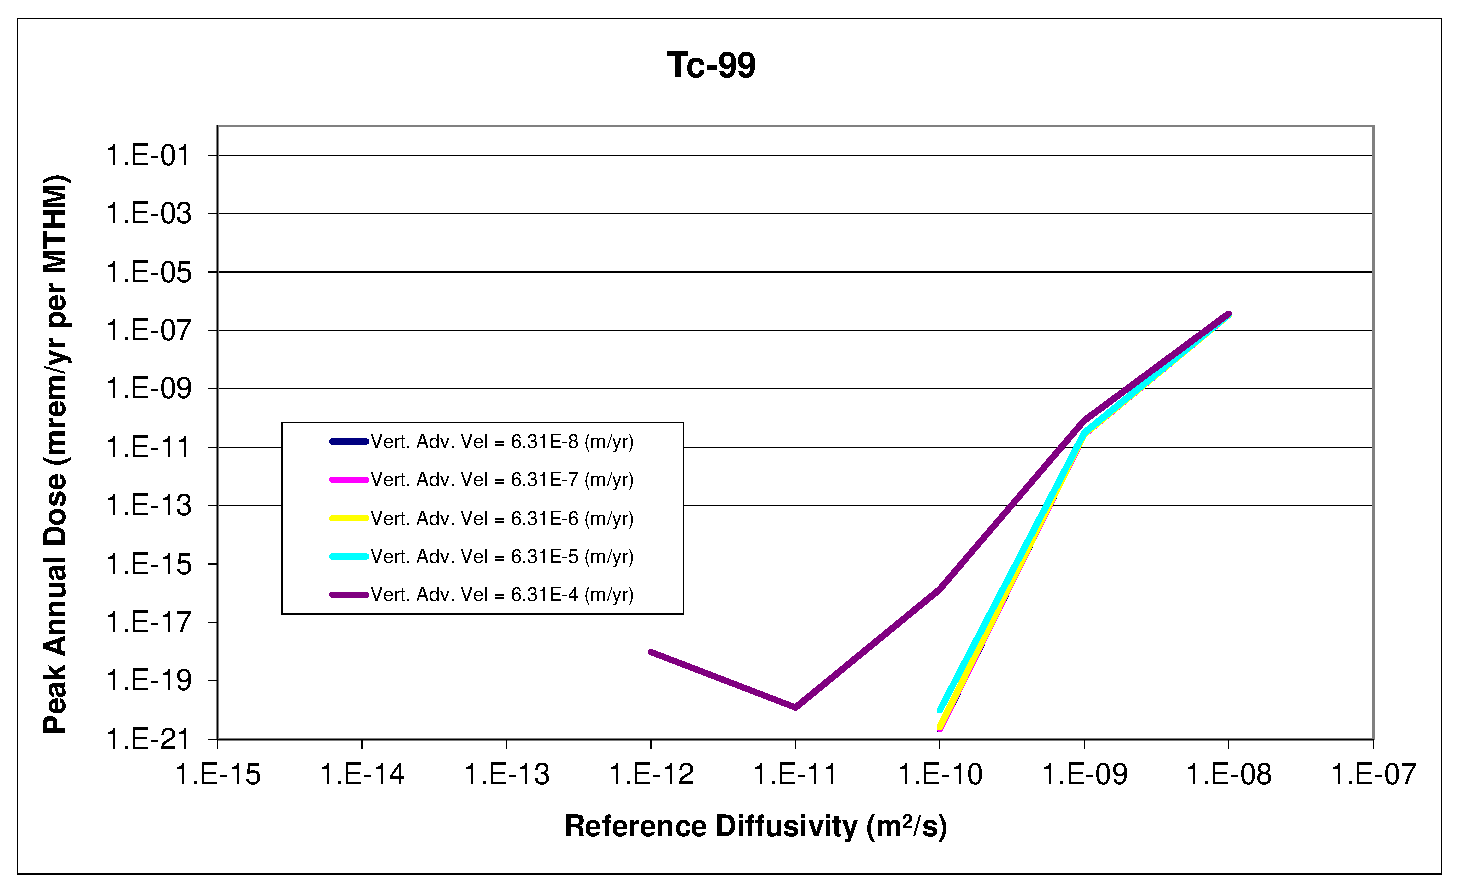
\includegraphics[width=0.8\textwidth]{AdvVelAndDiffCoeffEBSFail/Tc-99.eps}
\caption{$^{99}Tc$ 
shows a very weak influence on peak annual dose 
rate for low reference diffusivities, but a direct proportionality between 
dose and reference diffusivity above a threshold.}
\label{fig:VAdvVelTc99}
\end{figure}
\end{frame}

\begin{frame}[c]
  \frametitle{Case II : Vertical Advective Velocity and Diffusion Coefficient}
\begin{figure}[htp!]
\centering
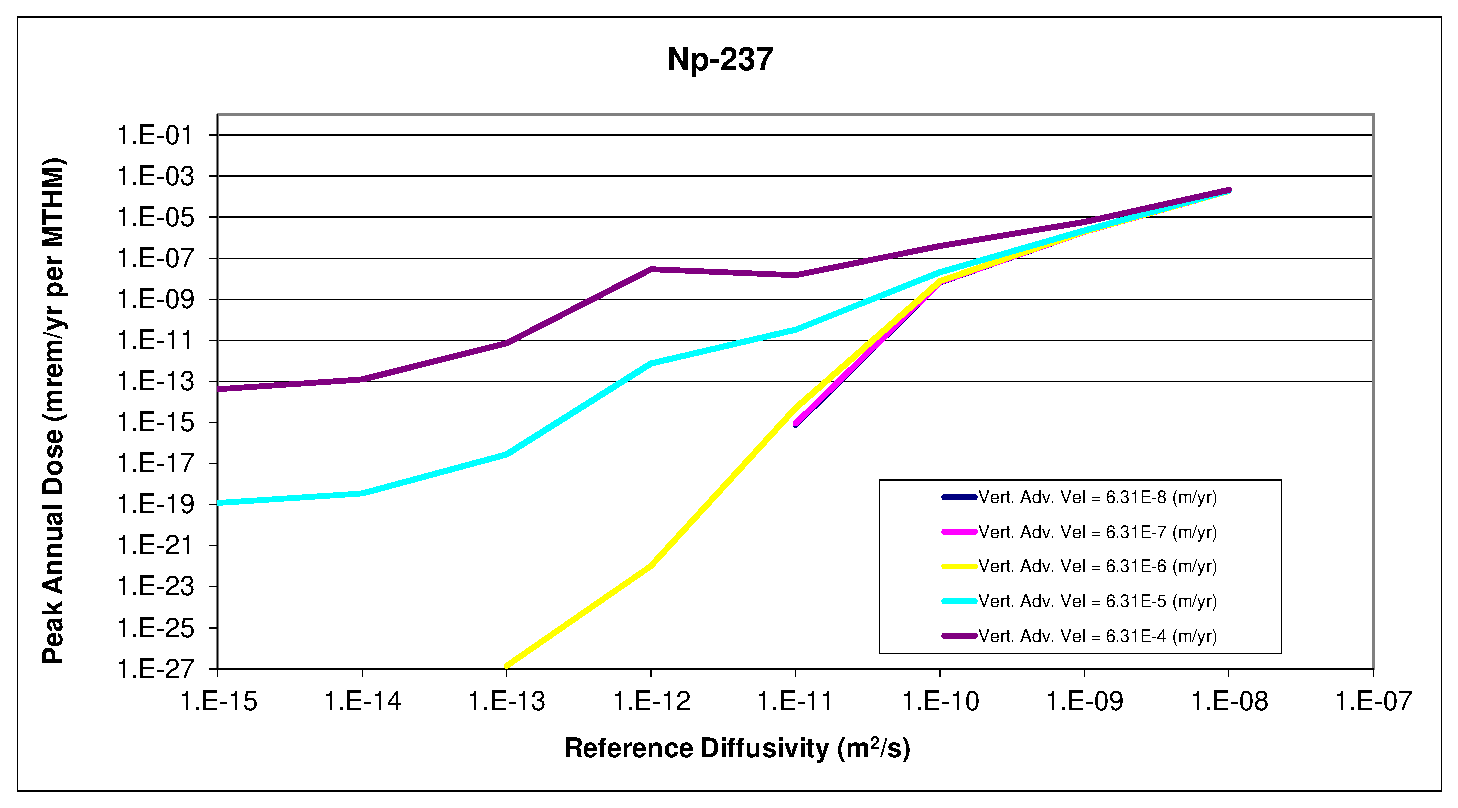
\includegraphics[width=0.8\textwidth]{AdvVelAndDiffCoeffEBSFail/Np-237.eps}
\caption{$^{237}Np$.
shows a very weak influence on peak annual dose 
rate for low reference diffusivities, but a direct proportionality between 
dose and reference diffusivity above a threshold.}
\label{fig:VAdvVelNp237}
\end{figure}
\end{frame}

\begin{frame}[c]
  \frametitle{Case II : Vertical Advective Velocity and Diffusion Coefficient}
\begin{figure}[htp!]
\centering
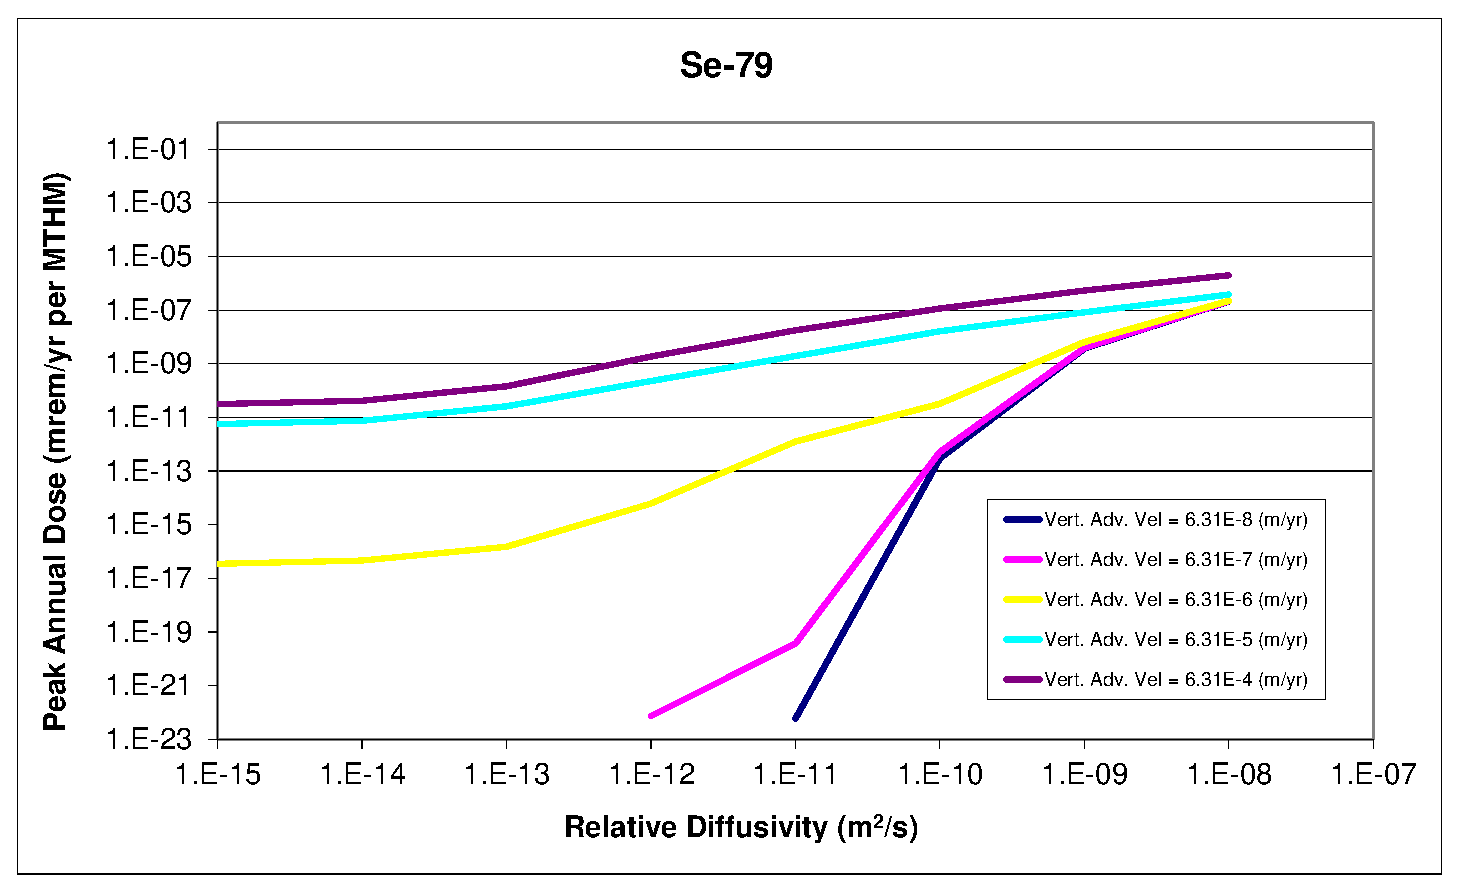
\includegraphics[width=0.8\textwidth]{AdvVelAndDiffCoeffEBSFail/Se-79.eps}
\caption{$^{79}Se$.
$Se$ is non sorbing, but solubility limited.  
For low vertical advective velocity, 
the system is diffusion dominated.}
\label{fig:VAdvVelSe79}
\end{figure}
\end{frame}


\begin{frame}[c]
  \frametitle{Case II : Vertical Advective Velocity and Diffusion Coefficient}
\begin{figure}[ht!]
\centering
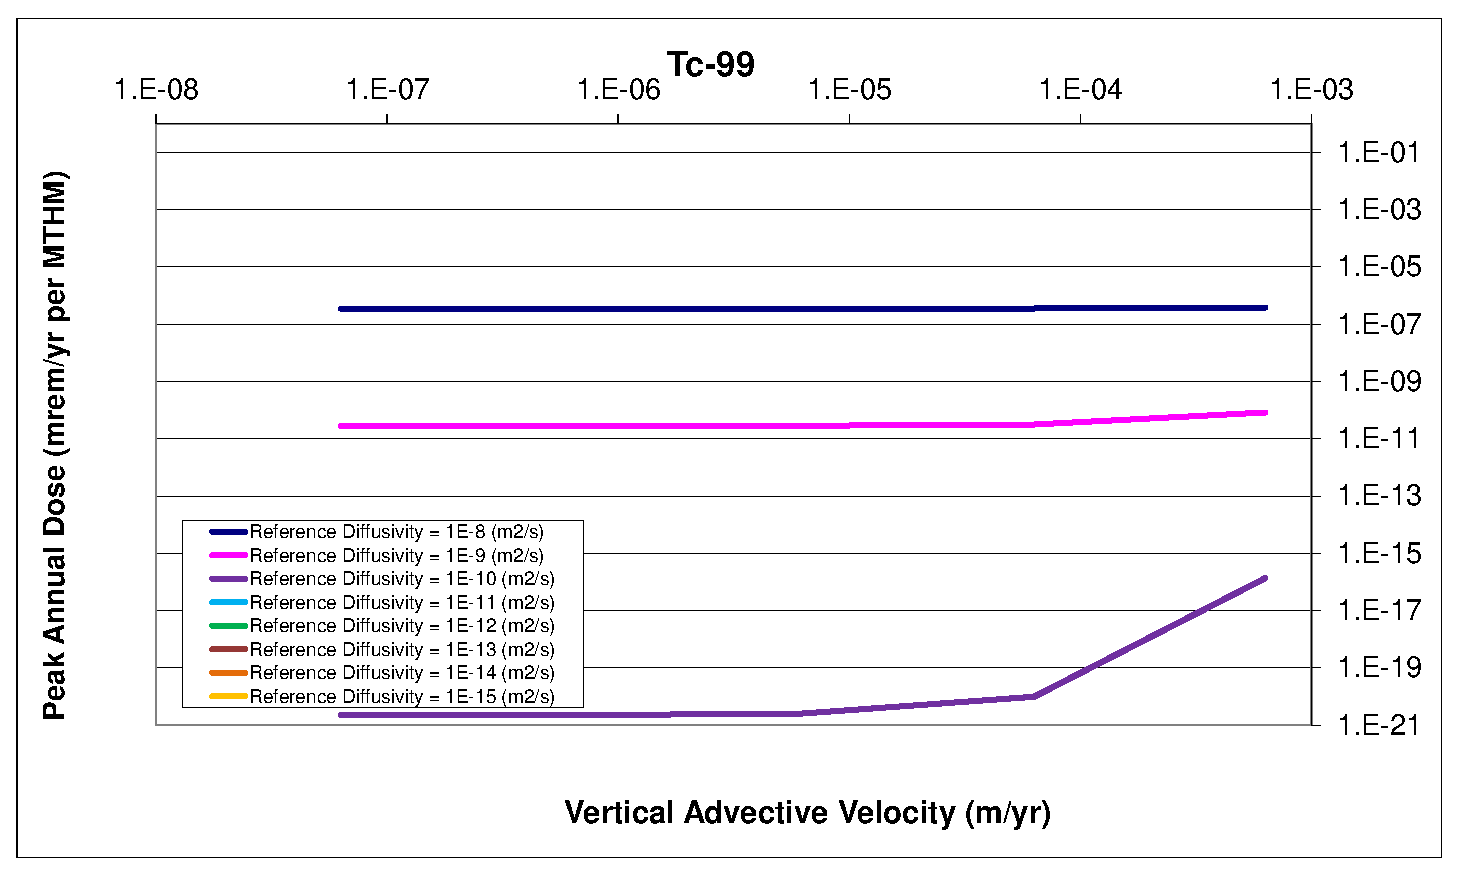
\includegraphics[width=0.8\textwidth]{AdvVelAndDiffCoeffEBSFail/Tc-99-VAdvVel.eps}
\caption{$^{99}Tc$.
shows a very weak influence on peak annual dose 
rate for low reference diffusivities, but a direct proportionality between 
dose and reference diffusivity above a threshold.}
\label{fig:VAdvVelTc99VAdvVel}
\end{figure}
\end{frame}


\begin{frame}[c]
  \frametitle{Case II : Vertical Advective Velocity and Diffusion Coefficient}
\begin{figure}[ht!]
\centering
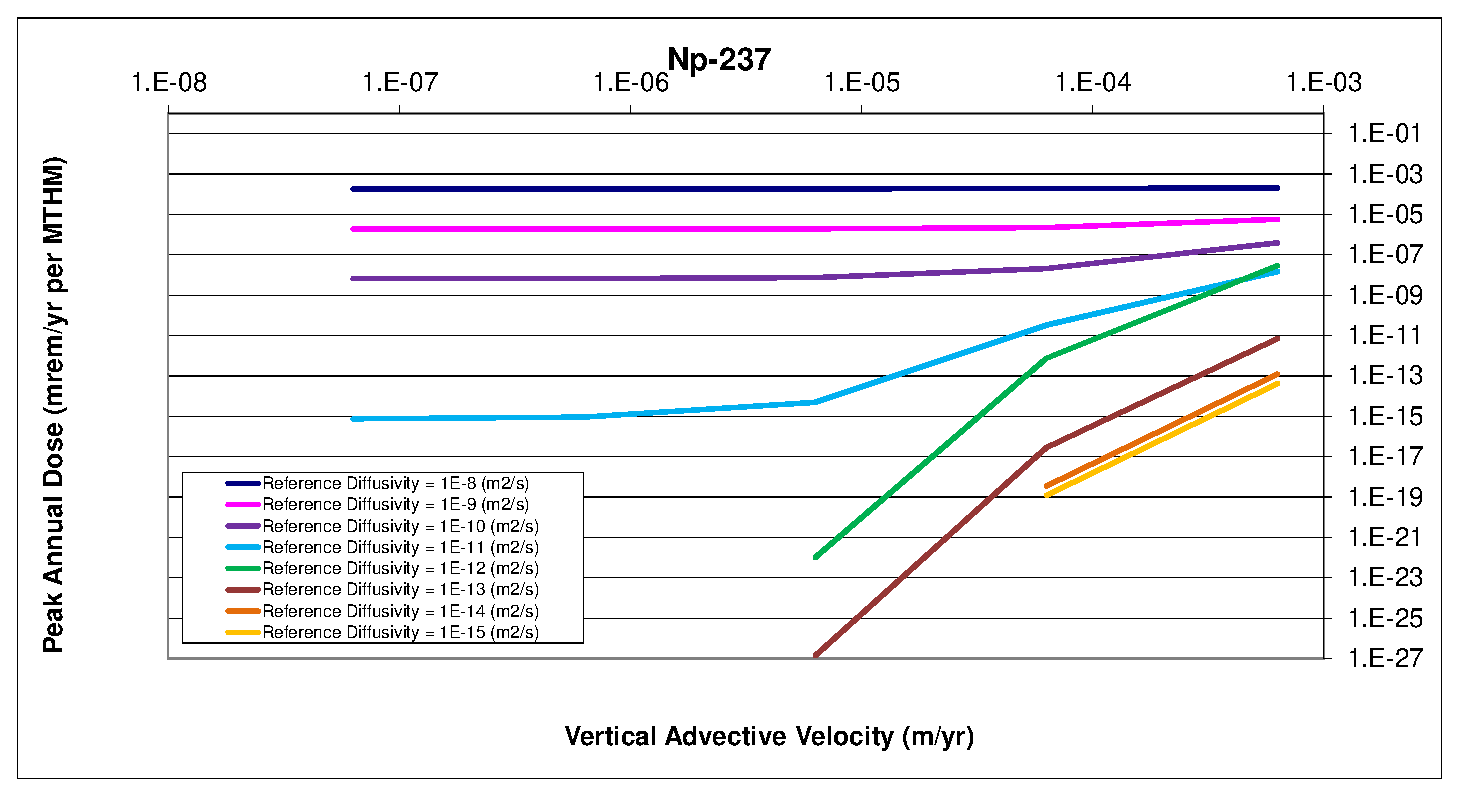
\includegraphics[width=0.8\textwidth]{AdvVelAndDiffCoeffEBSFail/Np-237-VAdvVel.eps}
\caption{$^{237}Np$.
shows a very weak influence on peak annual dose 
rate for low reference diffusivities, but a direct proportionality between 
dose and reference diffusivity above a threshold.}
\label{fig:VAdvVelNp237VAdvVel}
\end{figure}
\end{frame}

\begin{frame}[c]
  \frametitle{Case II : Vertical Advective Velocity and Diffusion Coefficient}
\begin{figure}[ht!]
\centering
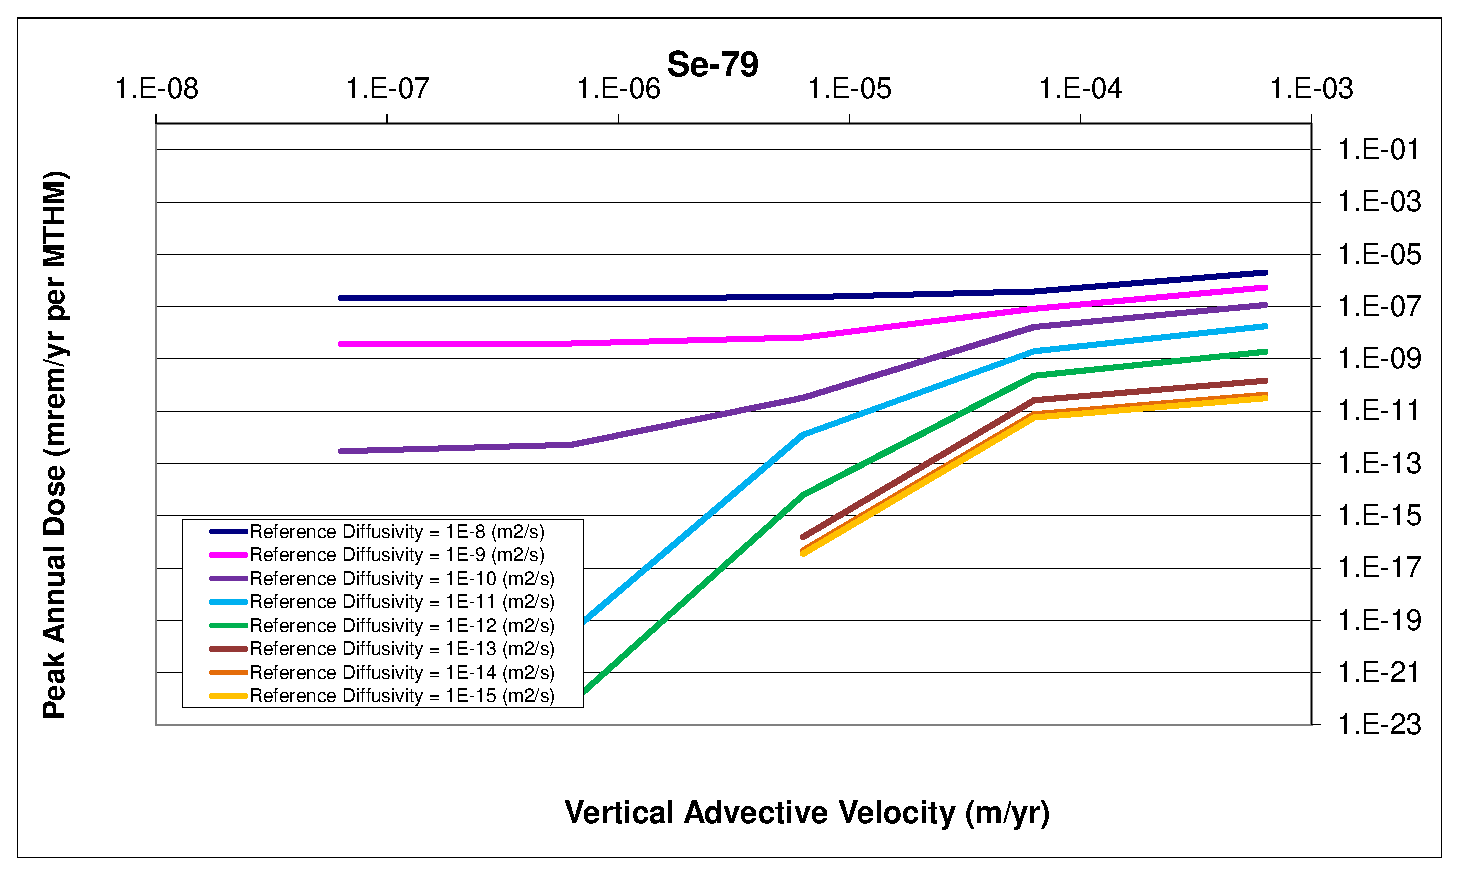
\includegraphics[width=0.8\textwidth]{AdvVelAndDiffCoeffEBSFail/Se-79-VAdvVel.eps}
\caption{$^{79}Se$.
$Se$ is non sorbing, but solubility limited.  
For high vertical advective 
velocity, the diffusivity remains important even in the advective regime as 
spreading facilitates transport in the presence of solubility limited transport. 
vertical advective velocity sensitivity.}
\label{fig:VAdvVelSe79VAdvVel}
\end{figure}
\end{frame}



\begin{frame}[c]
  \frametitle{Case III : Solubility Coefficient}
This study varied the solubility coefficients for each isotope in the simulation 
to help inform the effect of reprocessing on repository benefit for the clay 
repository scenario. The importance of the actinide contribution relative to the 
contribution from $^{129}I$, $^{79}Se$, and $^{99}Tc$ was of particular 
interest.
\end{frame}

\begin{frame}[c]
  \frametitle{Case III : Solubility Coefficient}
The dissolution behavior of a solute in an aqueous solutions is called its 
solubility. This behavior is limited by the solute's solubility limit, described  
by an equilibrium constant that depends upon temperature, water chemistry, and 
the properties of the element. The solubility constant for ordinary solutes, 
$K_s$ gives units of concentration, $[kg/m^3]$, and can be determined 
algebraically by the law of mass action which gives the partitioning at 
equilibrium between reactants and products.  For a reaction
\begin{align}
  cC + dD &= yY + zZ,
  \intertext{where}
  c,d,y,z  &= \mbox{ amount of respective constituent }[mol]\nonumber\\
  C,D  &= \mbox{ reactants }[-]\nonumber\\
  Y,Z  &= \mbox{ products }[-]\nonumber,
  \intertext{the law of mass action gives}
  K &= \frac{(Y)^y(Z)^z}{(C)^c(D)^d}
  \intertext{where}
  (X)  &= \mbox{ the equilibrium molal concentration of X }[mol/m^3]\nonumber\\
  K  &= \mbox{ the equilibrium constant }[-].\nonumber
  \label{massaction}
\end{align}
\end{frame}

\begin{frame}[c]
  \frametitle{Case III : Solubility Coefficient}
The equilibrium constant for many reactions are known, and can be found in 
chemical tables. Thereafter, the solubility constraints of a solution at 
equilibrium can be found algebraically.  In cases of salts that  dissociate in 
aqueous solutions, this equilibrium constant is called the salt's solubility 
product $K_{sp}$.
\end{frame}

\begin{frame}[c]
  \frametitle{Case III : Solubility Coefficient}
This equilibrium model, however, is only appropriate for dilute situations, and 
nondilute solutions at  partial equilibrium must be treated with an activity 
model by substituting the activities of the constituents  for their molal 
concentrations,
\begin{align}
  [X] &= \gamma_x(X)
  \intertext{where}
  [X]  &= \mbox{ activity of X }[-]\nonumber\\
  \gamma_x  &= \mbox{ activity coefficient of X}[-]\nonumber\\
  (X)  &= \mbox{ molal concentration of X}[mol/m^3]\nonumber
  \intertext{such that}
  IAP &= \mbox{ Ion Activity Product }[-].\nonumber\\
      &= \frac{[Y]^y[Z]^z}{[C]^c[D]^d}\\
  \label{IAP}
\end{align}
The ratio between the IAP and the equilibrium constant $(IAP/K)$ quantifies
the departure from equilibrium of a solution.  This information is useful during 
the transient stage in which a solute is first introduced to a solution. When 
$IAP/K<1$, the solution is undersaturated with respect to the products. When, 
conversely, $IAP/K>1$, the solution is oversaturated and precipitation of solids 
in the volume will occur. 
\end{frame}

\begin{frame}[c]
  \frametitle{Case III : Solubility Coefficient}
The solubility coefficients were varied in this simulation using a multiplier. 
The reference solubilities for each element were multiplied by the multiplier 
for each simulation group. This technique preserved relative solubility among 
  elements. Forty values of solubility coefficient multiplier were used to change 
the far field solubility. This did not alter any of the solubility in the
EDZ, WF, or Fast Path solubilities.

The values of the solubility multiplier were deliberately varied over many 
magnitudes, from $1\time10^{-9}$ through $5\times10^{10}$. This multiplier
multiplied the most likely values of solubility for each element, so 
the relative solubility between elements was preserved.
\end{frame}


\begin{frame}[c]
  \frametitle{Case III : Solubility Coefficient}
The results for varying the solubility coefficient were very straightforward.  
For solubility limits below a certain threshold, the dose releases were directly 
proportional to the solubility limit, indicating that the radionuclide 
concentration saturated the groundwater up to the solubility limit near the 
waste form.  For solubility limits above the threshold, however, further 
increase to the limit had no effect on the peak dose. This demonstrates the 
situation in which the solubility limit is so high that even complete 
dissolution of the waste inventory into the pore water is insufficient to reach 
the solubility limit.
\end{frame}

\begin{frame}[c]
  \frametitle{Case III : Solubility Coefficient}

In Figures \ref{fig:SolSumFactor} and \ref{fig:SolSum}, it is clear that for 
solubility constants lower than a threshold, the relationship between peak 
annual dose and solubility limit is strong.

\begin{figure}[ht]
\centering
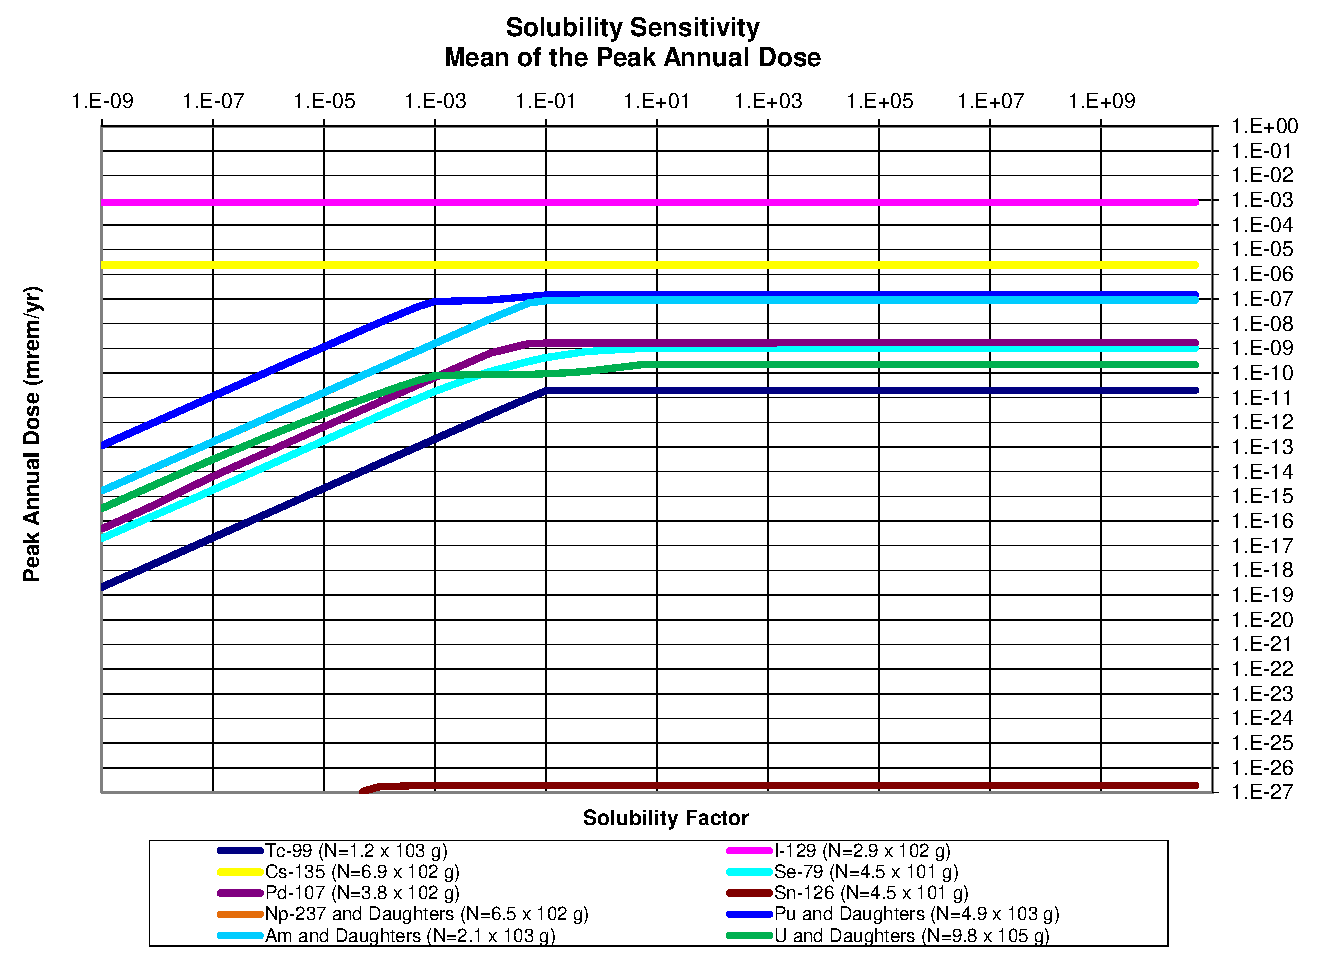
\includegraphics[width=\linewidth]{Solubility/Solubility_Summary_SolFactor.eps}
\caption{Solubility factor sensitivity. The peak annual dose due to an inventory, 
$N$, of each isotope.}
\label{fig:SolSumFactor}
\end{figure}
\end{frame}

\begin{frame}[c]
  \frametitle{Case III : Solubility Coefficient}

\begin{figure}[ht]
\centering
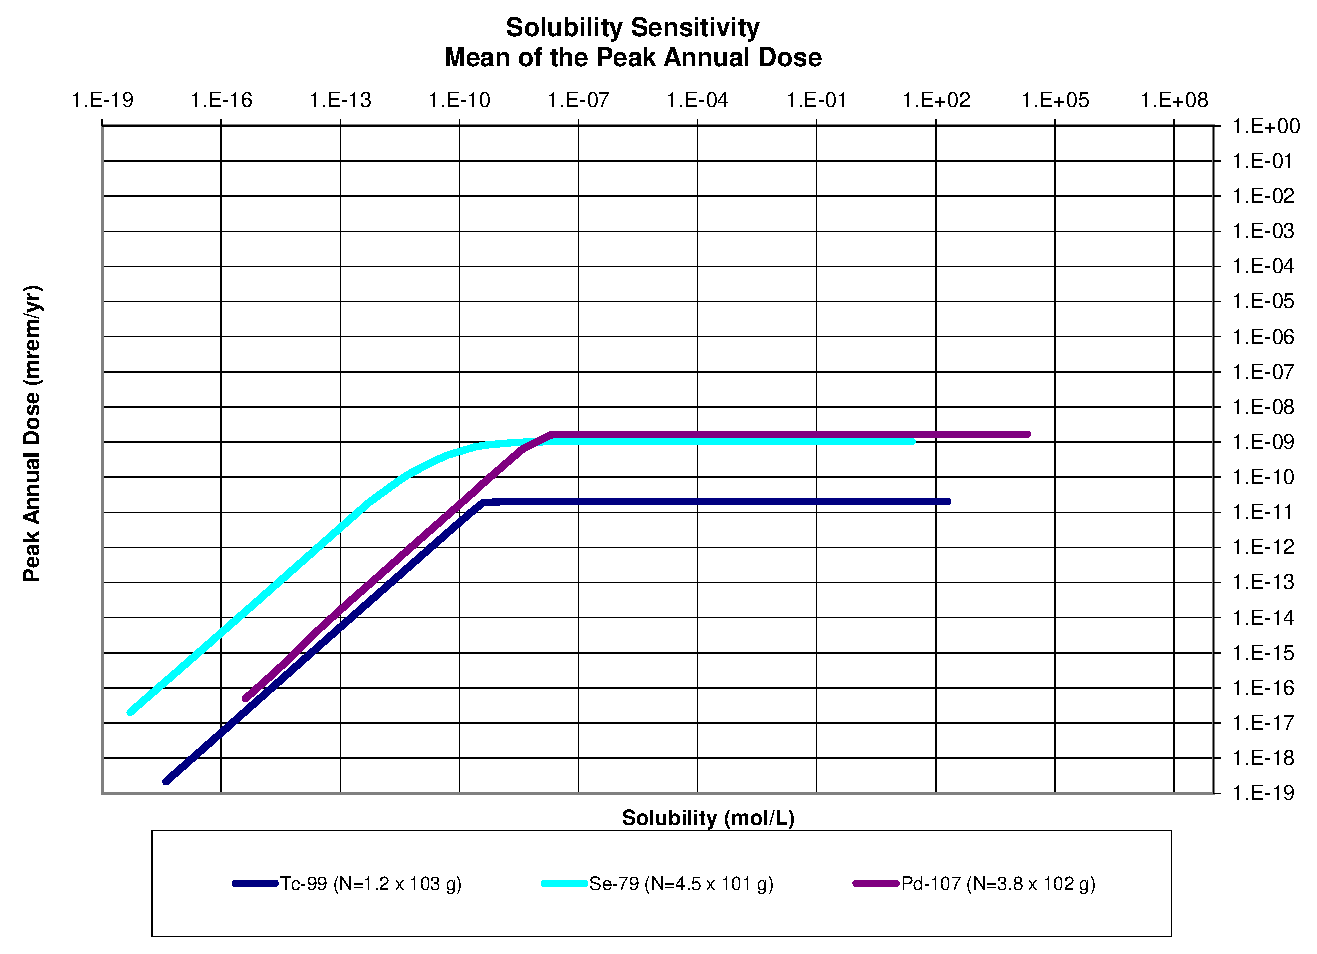
\includegraphics[width=\linewidth]{Solubility/Solubility_Summary_Sol.eps}
\caption{Solubility limit sensitivity. The peak annual dose due to an inventory, 
$N$, of each isotope.}
\label{fig:SolSum}
\end{figure}
\end{frame}



\begin{frame}[c]
  \frametitle{Case IV : Partition Coefficient}

This analysis investigated the peak dose rate contribution from various 
radionuclides to the partition coefficient of those radionuclides. 

The partition or distribution coefficient, $K_d$, relates the amount of contaminant adsorbed into the 
solid phase of the host medium to the amount of contaminant adsorbed into the 
aqueous phase of the host medium. It is a common empirical coefficient used to 
capture the effects of a number of retardation mechanisms. The coefficient 
$K_d$, in units of $[m^3\cdot kg^{-1}]$, is the ratio of the mass of contaminant in the 
solid to the mass of contaminant in the solution.
\end{frame}

\begin{frame}[c]
  \frametitle{Case IV : Partition Coefficient}
The retardation factor, $R_f$, which is the ratio between velocity of water through a 
volume and the velocity of a contaminant through that volume, can be expressed 
in terms of the partition coefficient,

\begin{align}
  R_f &= 1+\frac{\rho_b}{n_e}K_d
  \intertext{where}
  \rho_b &= ~~\mbox{bulk density}[kg\cdot m^{-3}]\nonumber
  \intertext{and}
  n_e &= ~~\mbox{effective porosity of the medium}[\%].\nonumber
\end{align}
\end{frame}

\begin{frame}[c]
  \frametitle{Case IV : Partition Coefficient}

The parameters in this model were all set to the default values except a multiplier 
applied to the partitioning $K_d$ coefficients.
\begin{table}[ht!]
\centering
\footnotesize{
\begin{tabular}{|l|l|l|r|r|}
\multicolumn{5}{c}{\textbf{Simulation Cases}}\\
\hline
\textbf{Case} & \textbf{Parameter} & \textbf{Units} & \textbf{Min. Value} & \textbf{Max. Value}\\
\hline
IV    & $K_{d,i}$    & $[m^3\cdot kg^{-1}]$       & $(1\times10^{-9})\langle K_{d,i}\rangle $    &  $(5\times10^{10})\langle K_{d,i}\rangle $ \\
\hline
\end{tabular}
\caption{Case IV varied the partitioning coefficient, $K_d$, multiplication 
  factor. This single parameter simulation case had 40 simulation 
groups of 100 realizations each.}
\label{tab:Cases}
}
\end{table}


\end{frame}

\begin{frame}[c]
  \frametitle{Case IV : Partition Coefficient}

\begin{figure}[ht]
\centering
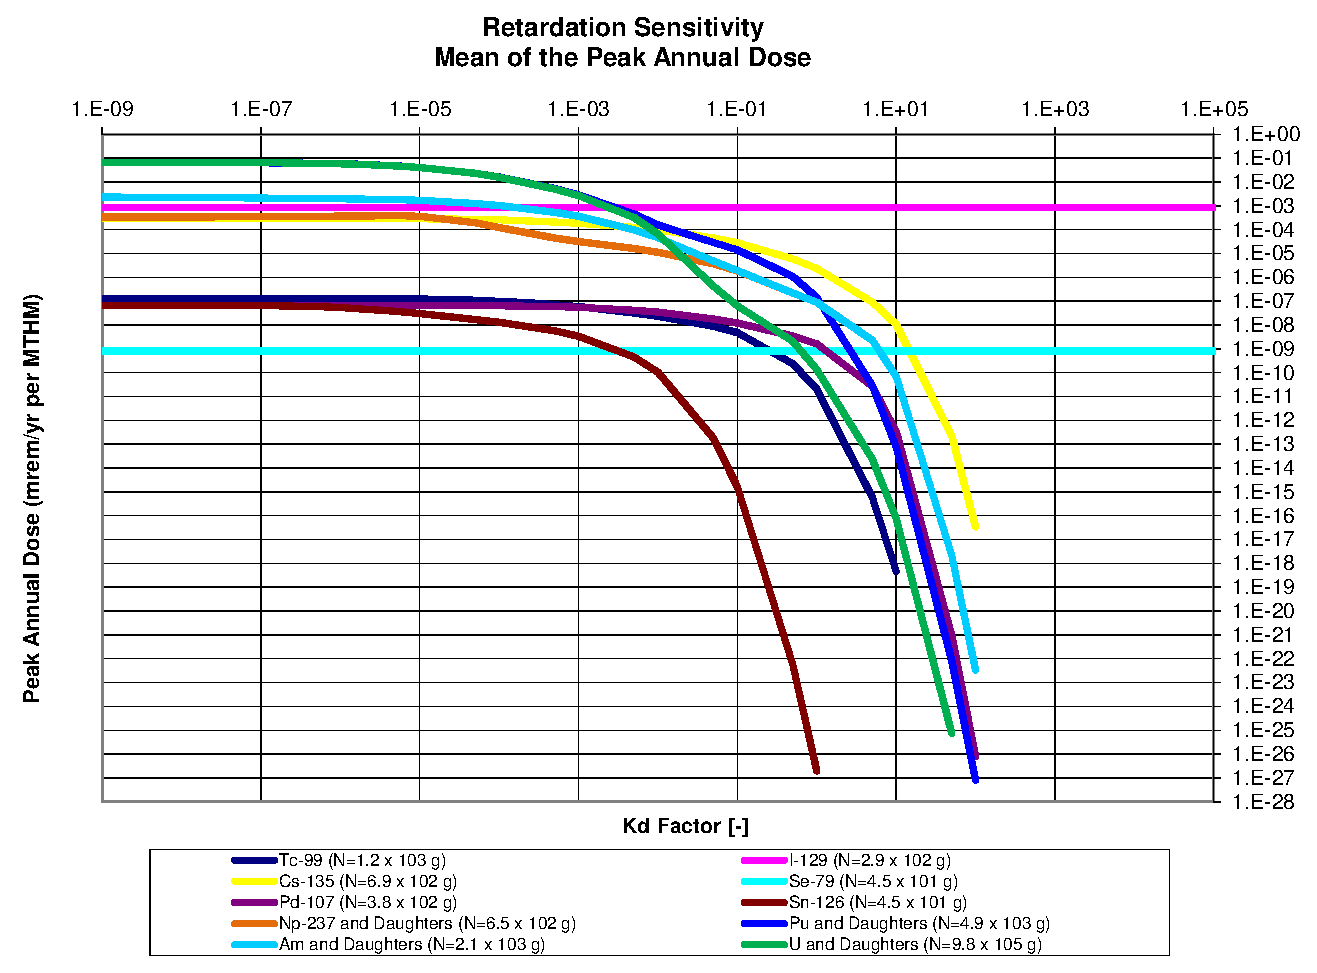
\includegraphics[width=0.8\textwidth]{Sorption/Retardation_Summary_kdFactor.eps}
\caption{
For retardation coefficients greater than a threshold, the 
relationship between peak annual dose and retardation coefficient is a strong 
inverse one. }
\label{fig:KdSumFactor}
\end{figure}
\end{frame}

\begin{frame}[c]
  \frametitle{Case IV : Partition Coefficient}

\begin{figure}[ht]
\centering
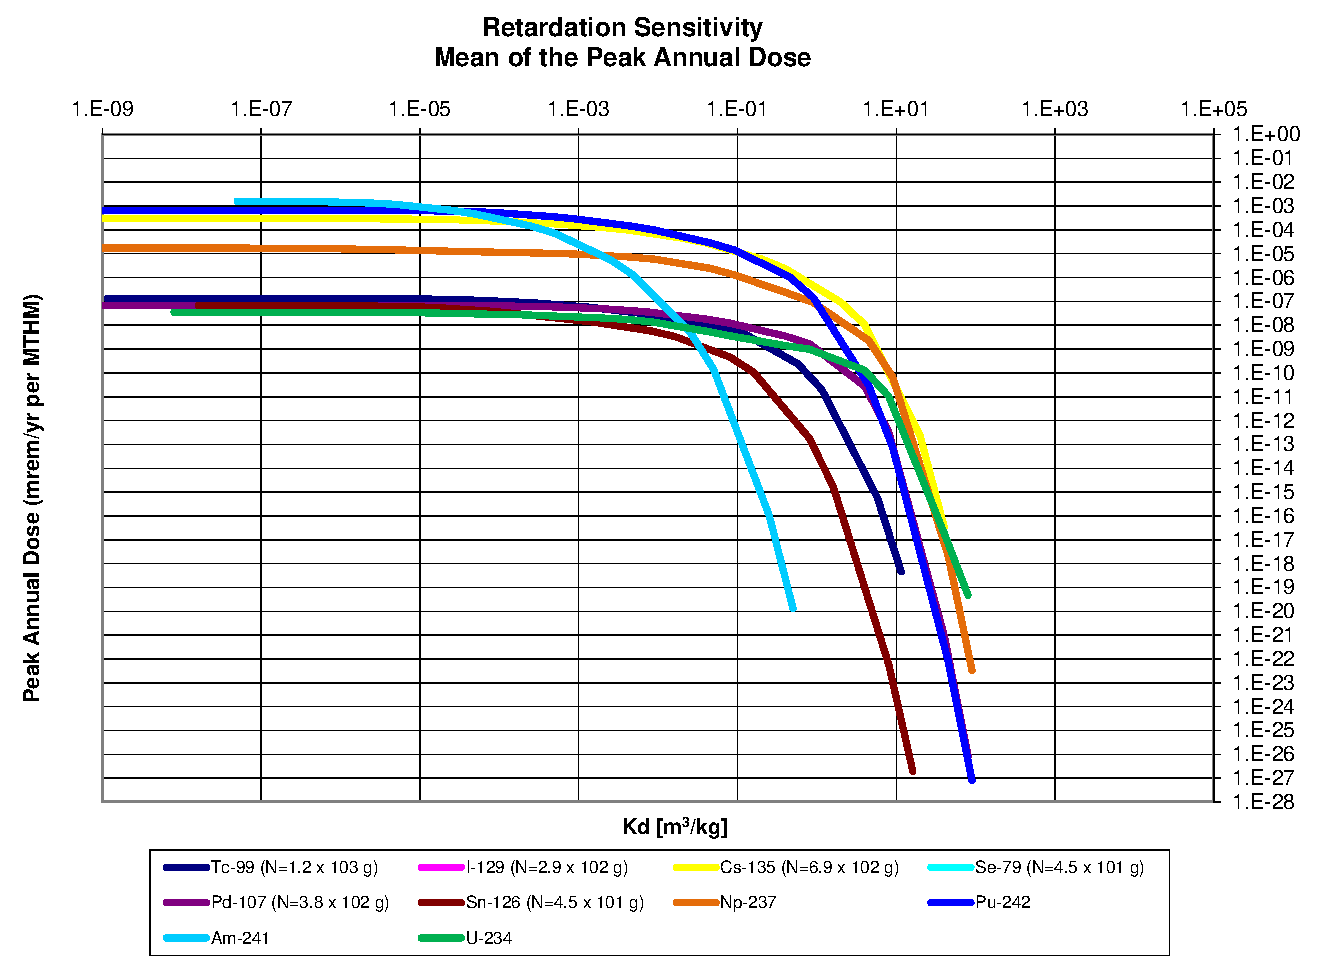
\includegraphics[width=0.8\textwidth]{Sorption/Retardation_Summary_kd.eps}
\caption{
For retardation coefficients greater than a threshold, the 
relationship between peak annual dose and retardation coefficient is a strong 
inverse one. }
\label{fig:KdSum}
\end{figure}
\end{frame}



\begin{frame}[c]
  \frametitle{Case V : Waste Form Degradation Rate and Inventory}
These runs varied the waste form degradation rate and the waste inventory mass 
factor.  There were forty runs corresponding to eight values of the waste form degradation 
rate and five values of the mass factor.

\begin{table}[ht!]
\centering
\footnotesize{
\begin{tabular}{|l|l|l|r|r|}
\multicolumn{5}{c}{\textbf{Simulation Cases}}\\
\hline
\textbf{Case} & \textbf{Parameter} & \textbf{Units} & \textbf{Min. Value} & \textbf{Max. Value}\\
\hline
V     & $R_{WFDeg.}$           & $[yr^{-1}]$       & $10^{-9}$    &  $10^{-2}$ \\
      & Inventory              & [MTHM]         & $10^{-4}$    &  $10^1$ \\
\hline
\end{tabular}
\caption{Each dual and single parameter simulation case had 40 simulation 
groups of 100 realizations each.}
\label{tab:Cases}
}
\end{table}


\end{frame}

\begin{frame}[c]
  \frametitle{Case V : Waste Form Degradation Rate and Inventory}

Safety indicators for post closure repository performance have been developed by 
the \gls{UFD} campaign which utilize the inventory multiplier that was varied in 
this study \cite{nutt_generic_2009}. These indicators are normalized by a 
normalization factor (100 mrem/yr) recommended by the \gls{IAEA} as the limit to 
``relevant critical members of the public'' \cite{iaea_international_1996}. The functional form for 
this safety indicator for a single waste category, \gls{HLW}, is just 

\begin{align}
SI_{G} &= \left(\frac{\sum_{i=1}^{N}D_{G,i}(I_i, F_{d})}{100mrem/yr}\right)[GWe/yr].
\label{indicator}
\intertext{where}
SI_{G} &= \mbox{Safety indicator for disposal in media type G}[GWe/yr]\nonumber\\
N &= \mbox{Number of key radionuclides considered in this indicator}\nonumber\\
D_{G,i} &= \mbox{Peak dose rate from isotope i in media type G}[mrem/yr]\nonumber\\
F_{d} &= \mbox{Fractional waste form degradation rate}[1/yr].\nonumber
\end{align}
\end{frame}

\begin{frame}[c]
  \frametitle{Case V : Waste Form Degradation Rate and Inventory}
\begin{figure}[ht!]
\centering
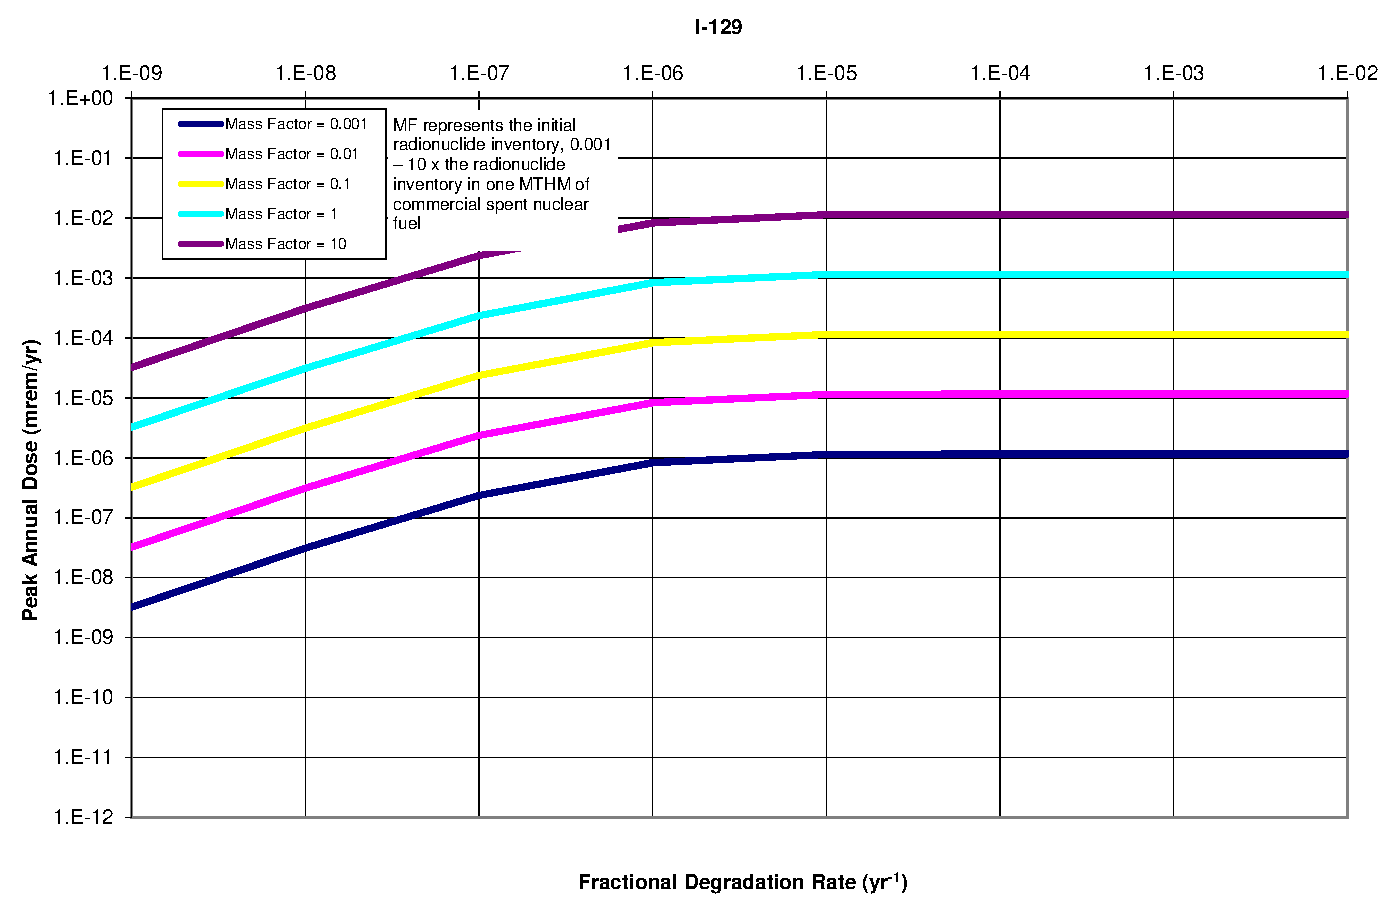
\includegraphics[width=0.8\textwidth]{WFDegAndInv/I-129.eps}
\caption{
Highly soluble and non-sorbing $^{129}I$ demonstrates a direct proportionality between dose rate and 
fractional degradation rate until a turnover where other natural system 
parameters dampen transport.} 
\label{fig:WFDegI129}
\end{figure}
\end{frame}

\begin{frame}[c]
  \frametitle{Case V : Waste Form Degradation Rate and Inventory}

\begin{figure}[ht!]
\centering
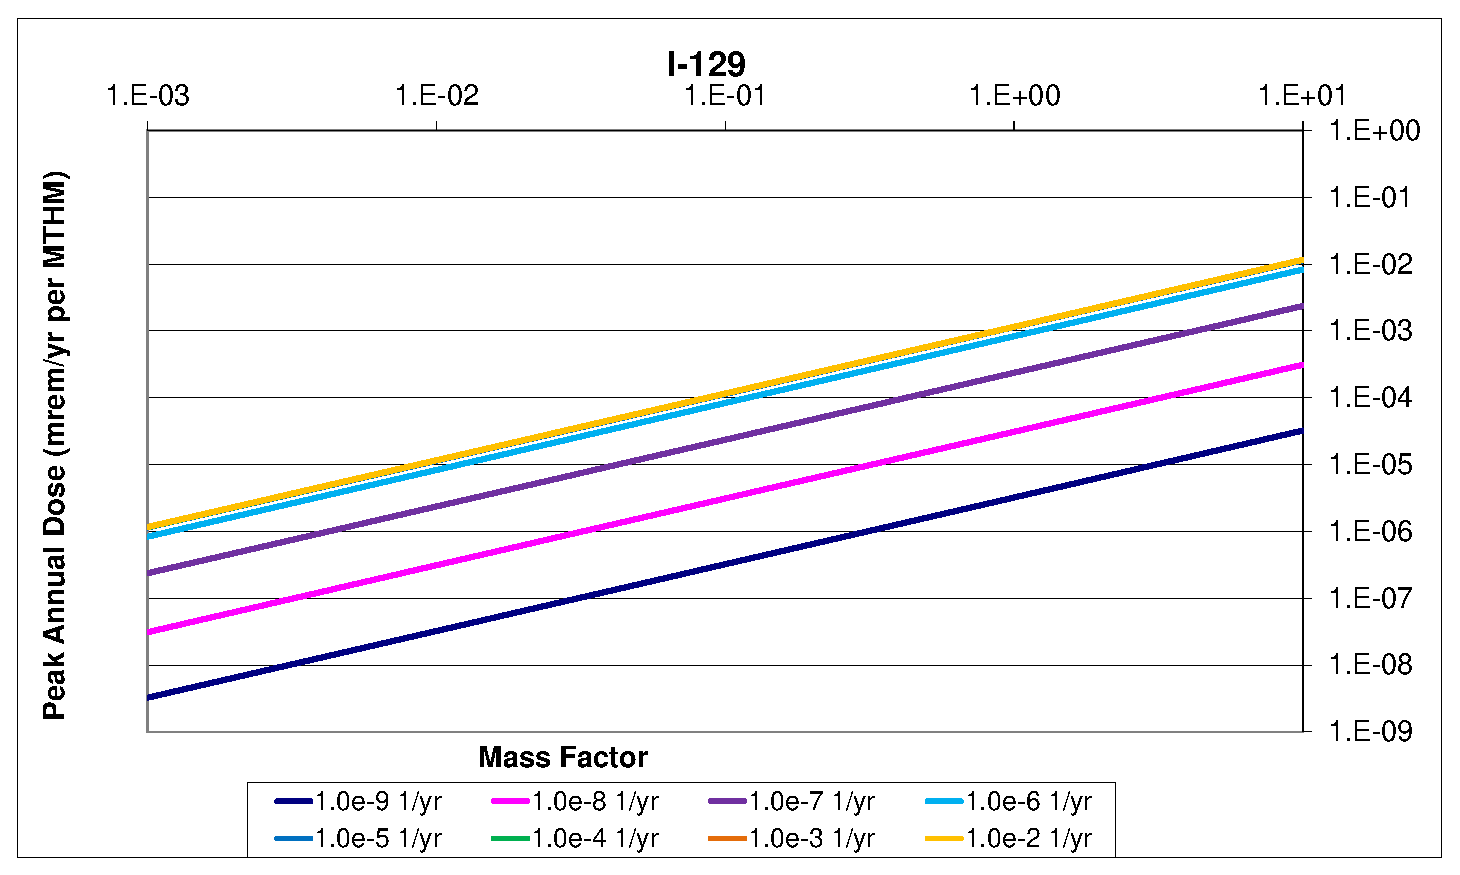
\includegraphics[width=0.8\textwidth]{WFDegAndInv/I-129-MF.eps}
\caption{
Highly soluble and non-sorbing $^{129}I$ domonstrates a direct 
proportionality to the inventory multiplier.}
\label{fig:WFDegI129MF}
\end{figure}
\end{frame}

\begin{frame}[c]
  \frametitle{Case V : Waste Form Degradation Rate and Inventory}
\begin{figure}[ht!]
\centering
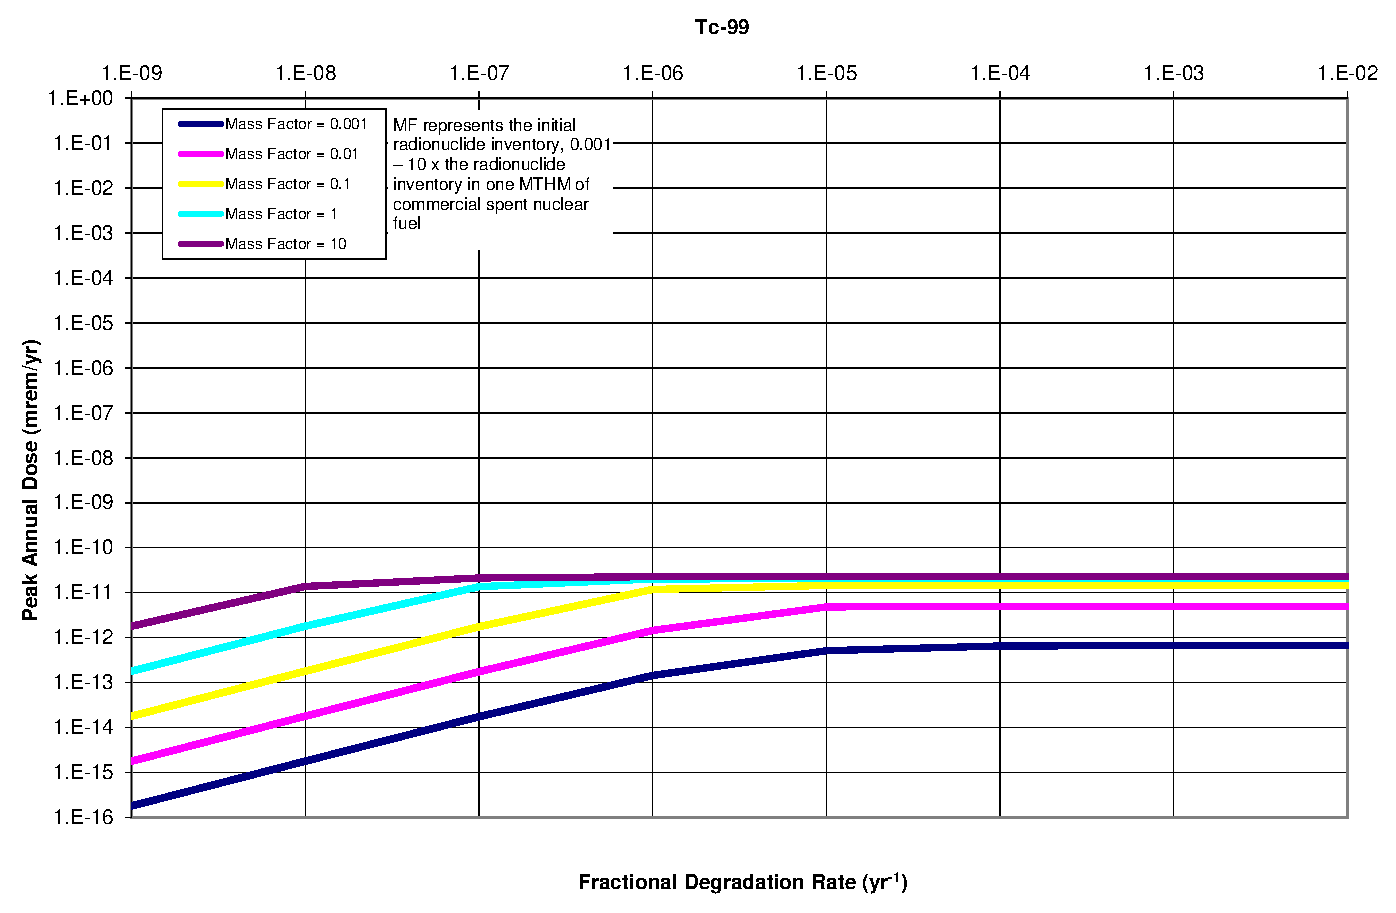
\includegraphics[width=0.8\textwidth]{WFDegAndInv/Tc-99.eps}
\caption{
Solubility limited and sorbing $^{99}Tc$ demonstrates a stronger turnover and direct proportionality 
to fractional degradation rate until attuation by its solubility limit and other 
natural system parameters. } 
\label{fig:WFDegTc99}
\end{figure}
\end{frame}

\begin{frame}[c]
  \frametitle{Case V : Waste Form Degradation Rate and Inventory}

\begin{figure}[ht!]
\centering
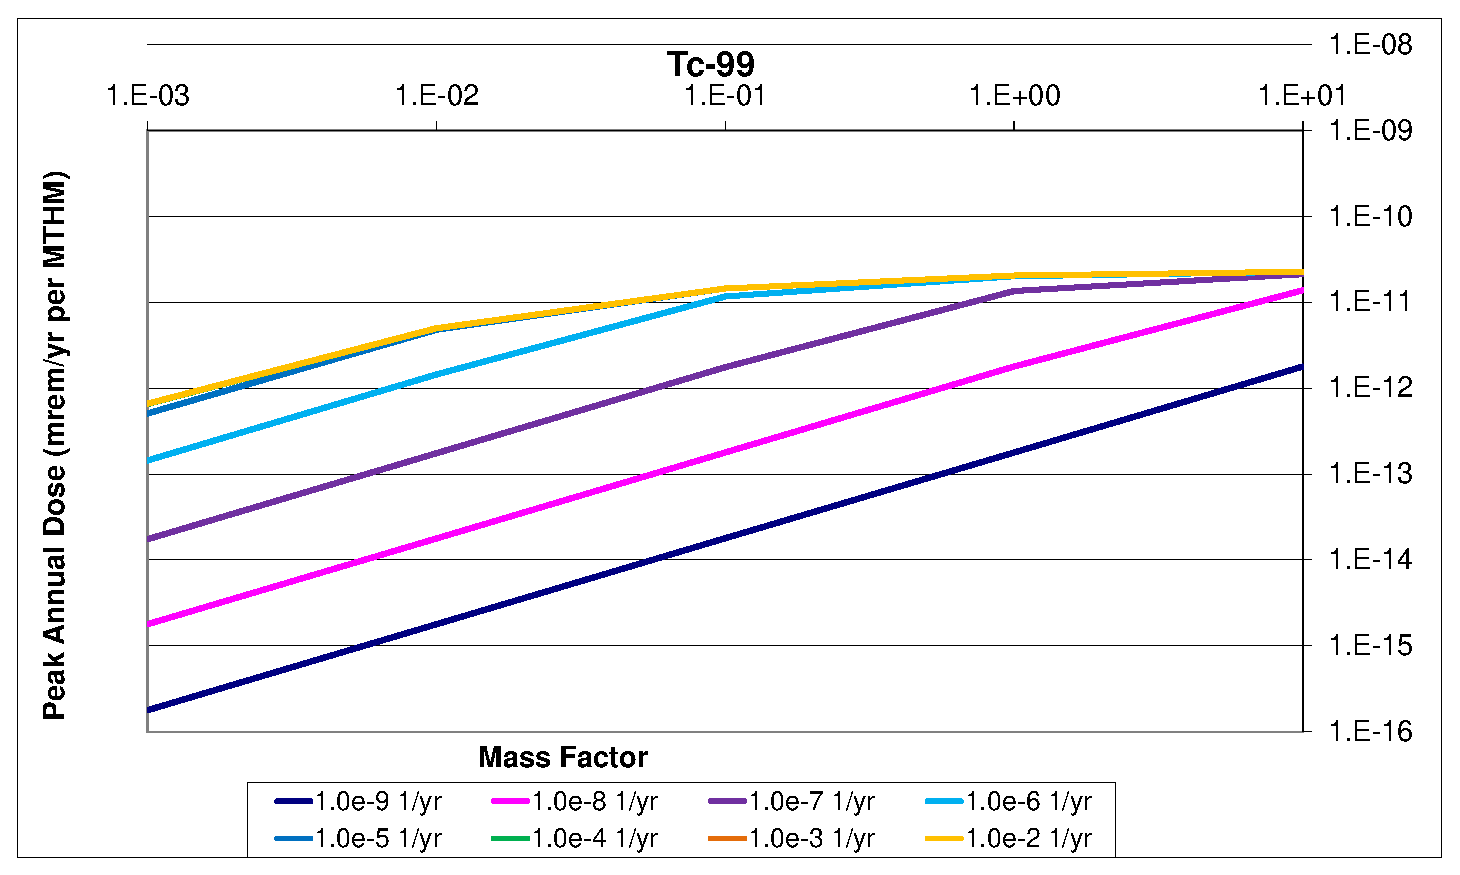
\includegraphics[width=0.8\textwidth]{WFDegAndInv/Tc-99-MF.eps}
\caption{
  Solubility limited and sorbing $^{99}Tc$ demonstrates a direct proportionality 
to fractional degradation rate until attuation by its solubility limit and other 
natural system parameters. } 
\label{fig:WFDegTc99MF}
\end{figure}

\end{frame}

\begin{frame}[c]
  \frametitle{Case V : Waste Form Degradation Rate and Inventory}

\begin{figure}[ht!]
\centering
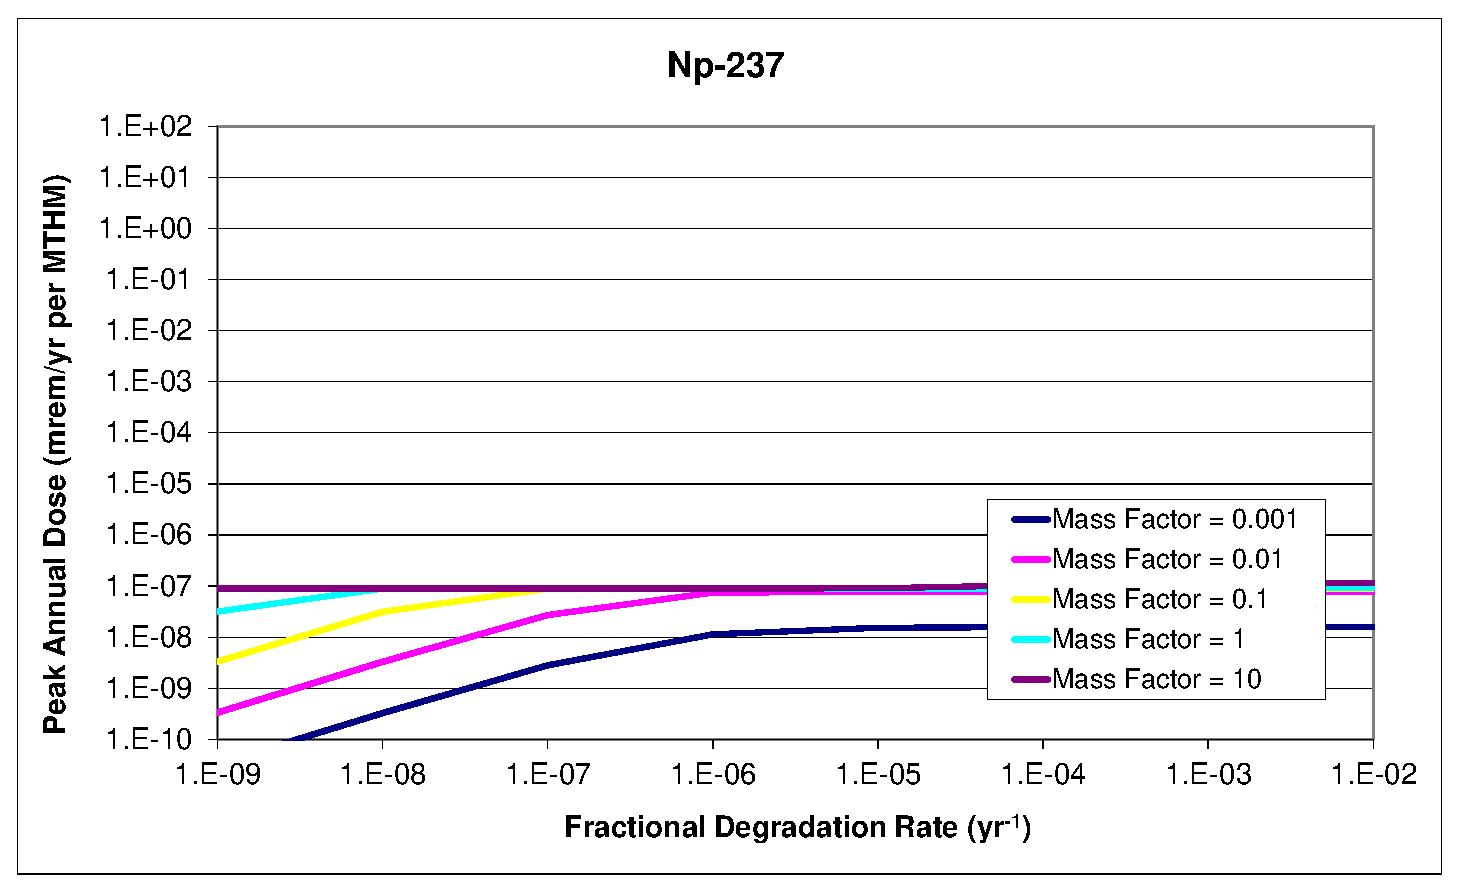
\includegraphics[width=0.8\textwidth]{WFDegAndInv/Np-237.eps}
\caption{
  Solubility limited and sorbing $^{237}Np$ demonstrates a direct proportionality 
to fractional degradation rate until attuation by its solubility limit and other 
natural system parameters. } 
\label{fig:WFDegNp237}
\end{figure}
\end{frame}

\begin{frame}[c]
  \frametitle{Case V : Waste Form Degradation Rate and Inventory}

\begin{figure}[ht!]
\centering
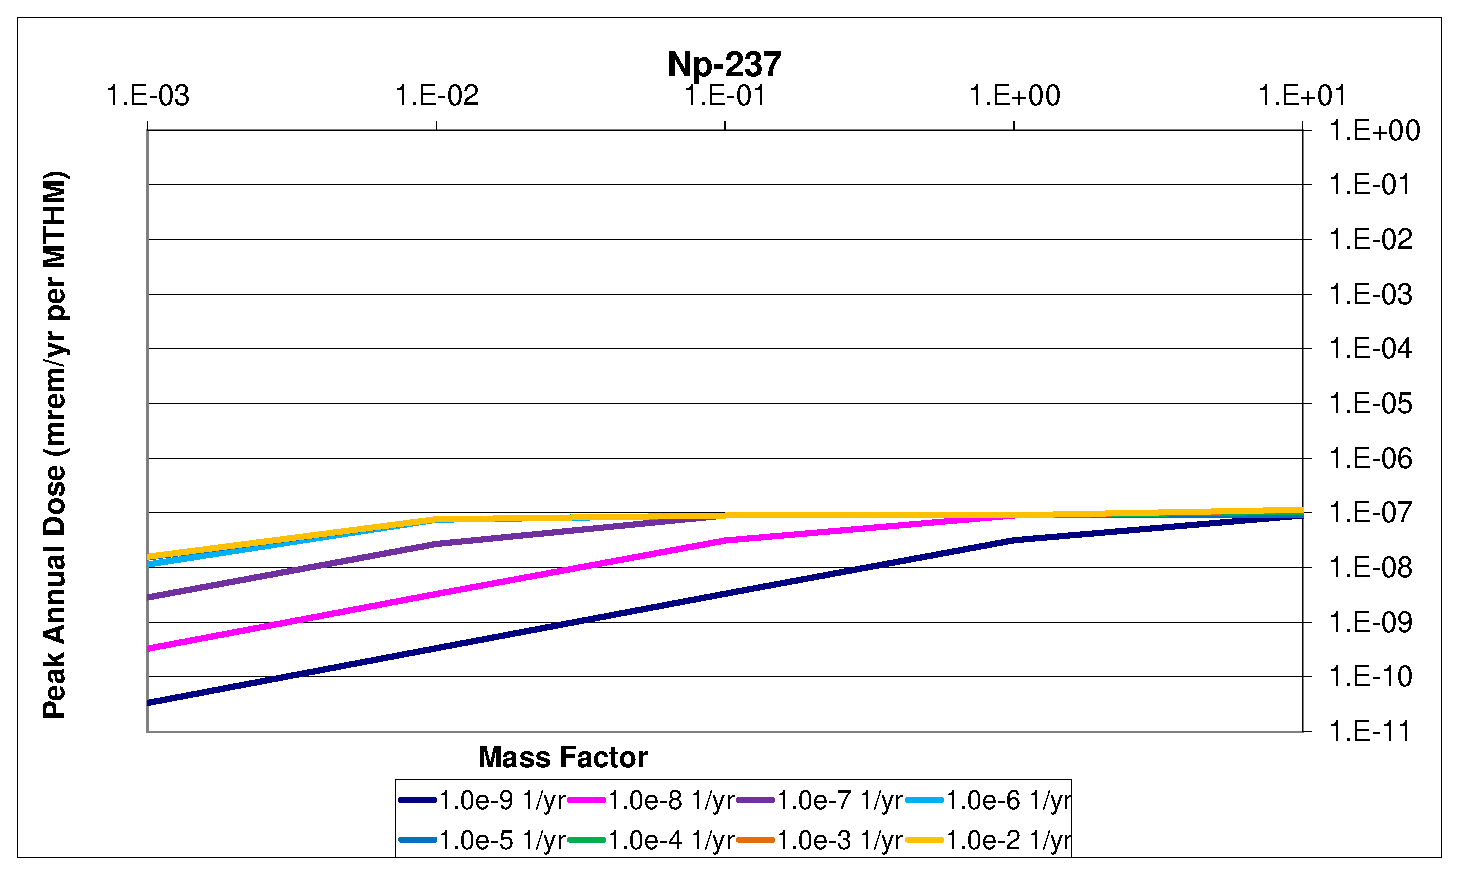
\includegraphics[width=0.8\textwidth]{WFDegAndInv/Np-237-MF.eps}
\caption{
  Solubility limited and sorbing $^{237}Np$ demonstrates a direct proportionality 
to fractional degradation rate until attuation by its solubility limit and other 
natural system parameters. } 
\label{fig:WFDegNp237MF}
\end{figure}

\end{frame}



\begin{frame}[c]
  \frametitle{Case VI : Waste Package Failure Time and Diffusion Coefficient}

The time of waste package failure was not expected to greatly effect the 
magnitude of the mean of the peak doses except for cases in which waste package failure times 
exceeded the half lives of dominant dose-contributing nuclides. 
That is, since the dominant dose-contributing 
radionuclides for the reference case are quite long lived ($^{129}I$, etc.), 
all but the longest reasonable waste package containment lifetime is overwhelmed by 
the half life of the dominant radionuclides. The long time scales of 
radionuclide release was expected to render the the waste package lifetime 
irrelevant if it was shorter than a million years. 
\end{frame}

\begin{frame}[c]
  \frametitle{Case VI : Waste Package Failure Time and Diffusion Coefficient}
Though the model contains a unit cell-type model, it is possible to determine, 
in post processing, the results of a simulation with temporally heterogeneous 
failures among waste packages. That is, by a weighted sum of the time histories 
of the no-fail case and the all-fail case, it is possible to mimic a 
time-varying failure among the many waste packages. 

\end{frame}

\begin{frame}[c]
  \frametitle{Case VI : Waste Package Failure Time and Diffusion Coefficient}

To investigate the effect of the waste package failure time, it was varied over 
five magnitudes from one thousand to ten million years. Simultaneously, the reference 
diffusivity was varied over the eight magnitudes between $1\times10^{-8}$ and 
$1\times10^{-15}$ in order to determine the correlation between increased 
radionuclide mobility and the waste package lifetime. 

\end{frame}

\begin{frame}[c]
  \frametitle{Case VI : Waste Package Failure Time and Diffusion Coefficient}

For the clay repository, the waste package failure time is entirely irrelevant 
until waste package failure times reach the million or ten million year time 
scale. 

\begin{figure}[ht!]
\centering
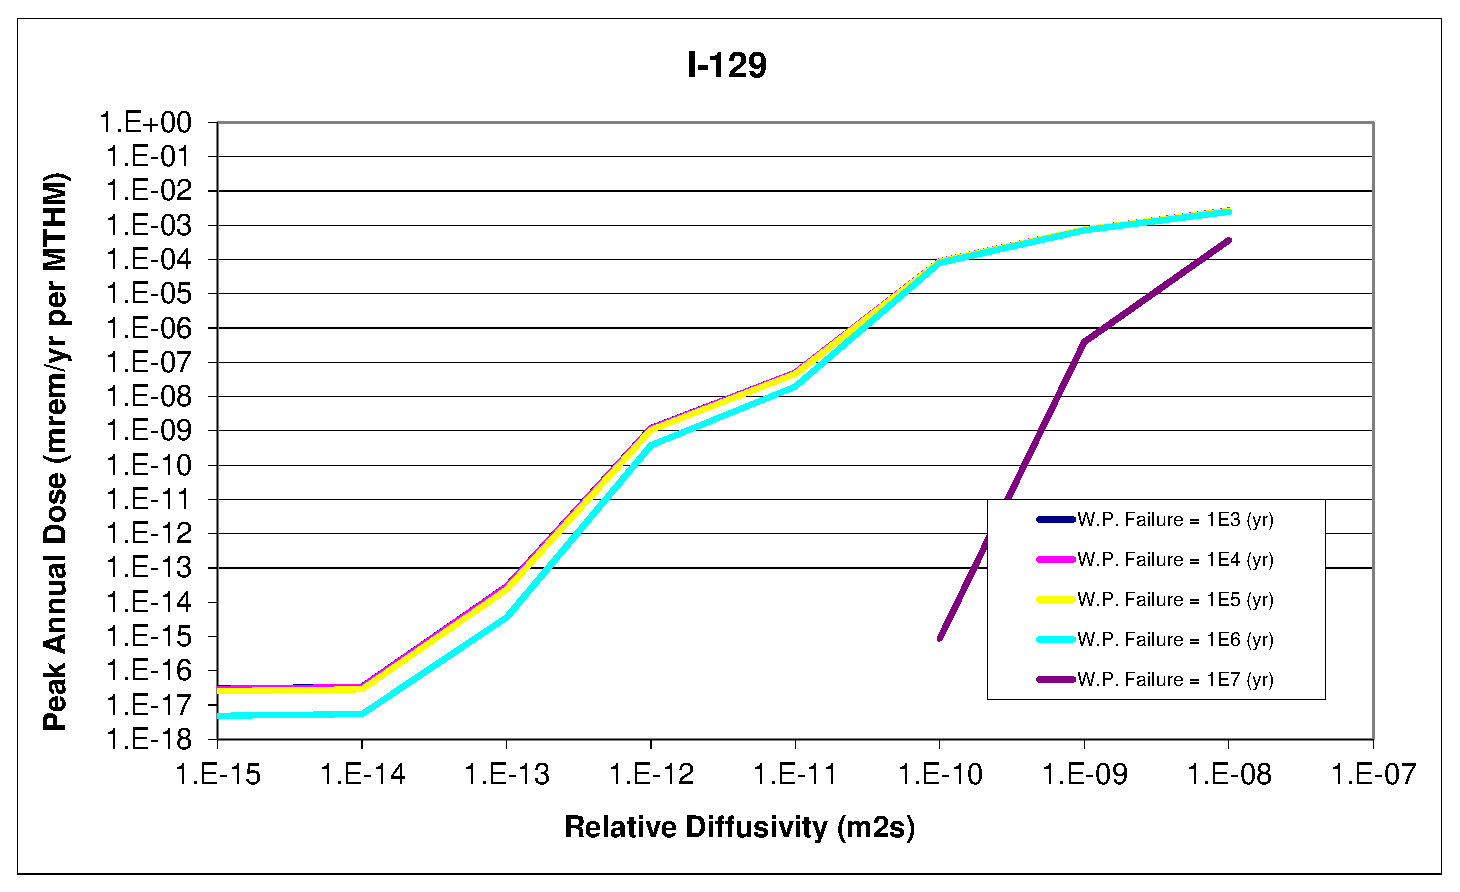
\includegraphics[width=\linewidth]{WPFailExtended/I-129.eps}
\caption{$^{129}I$ waste package failure time sensitivity. }
\label{fig:WPFailI129}
\end{figure}
\end{frame}

\begin{frame}[c]
  \frametitle{Case VI : Waste Package Failure Time and Diffusion Coefficient}

\begin{figure}[ht!]
\centering
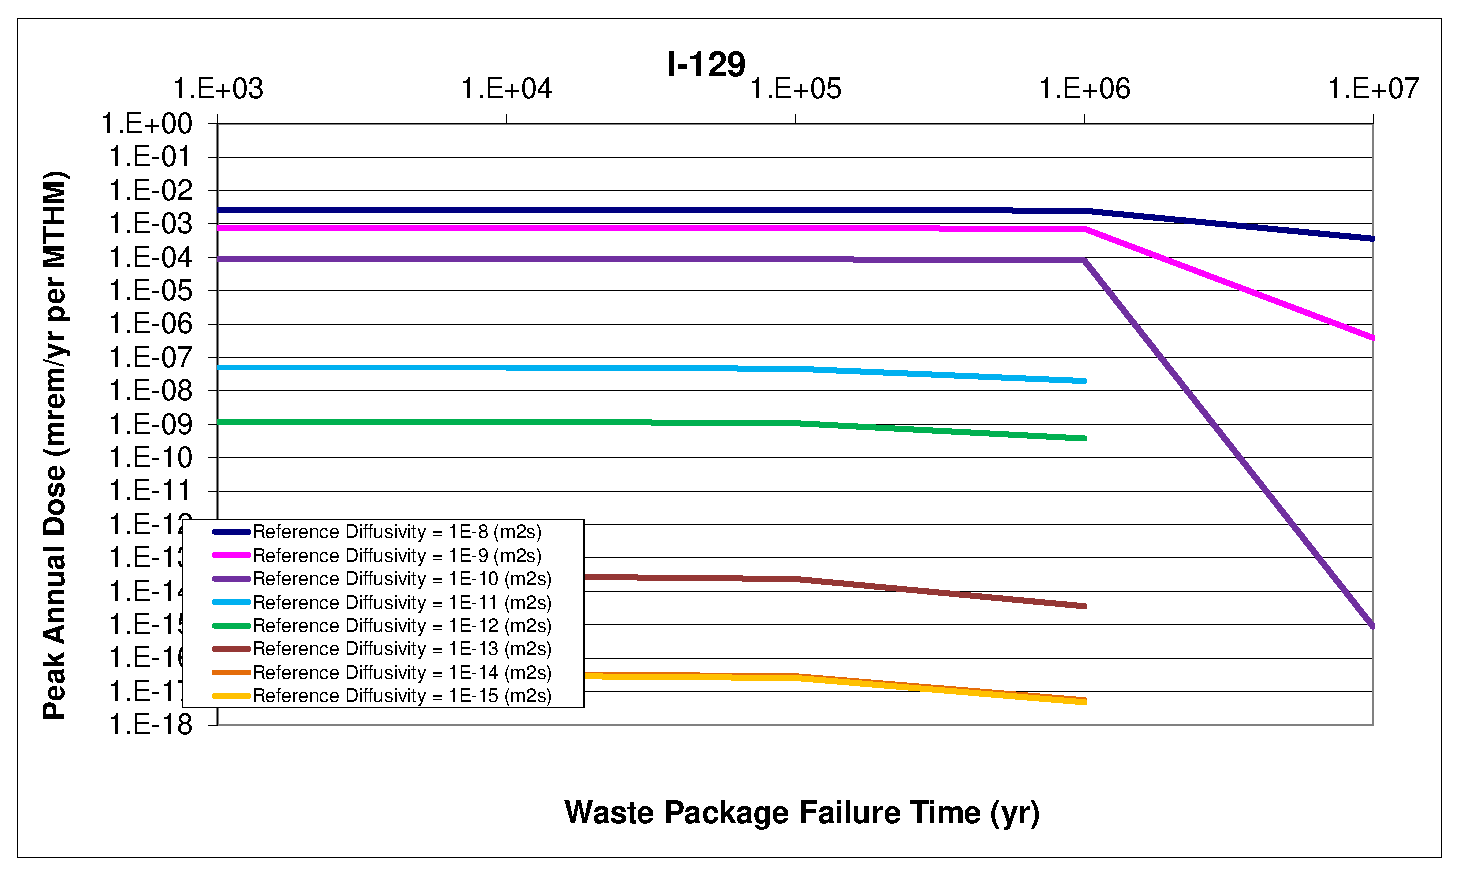
\includegraphics[width=\linewidth]{WPFailExtended/I-129-WPFail.eps}
\caption{$^{129}I$ waste package failure time sensitivity. }
\label{fig:WPFailI129}
\end{figure}
\end{frame}

\begin{frame}[c]
  \frametitle{Case VI : Waste Package Failure Time and Diffusion Coefficient}

\begin{figure}[ht!]
\centering
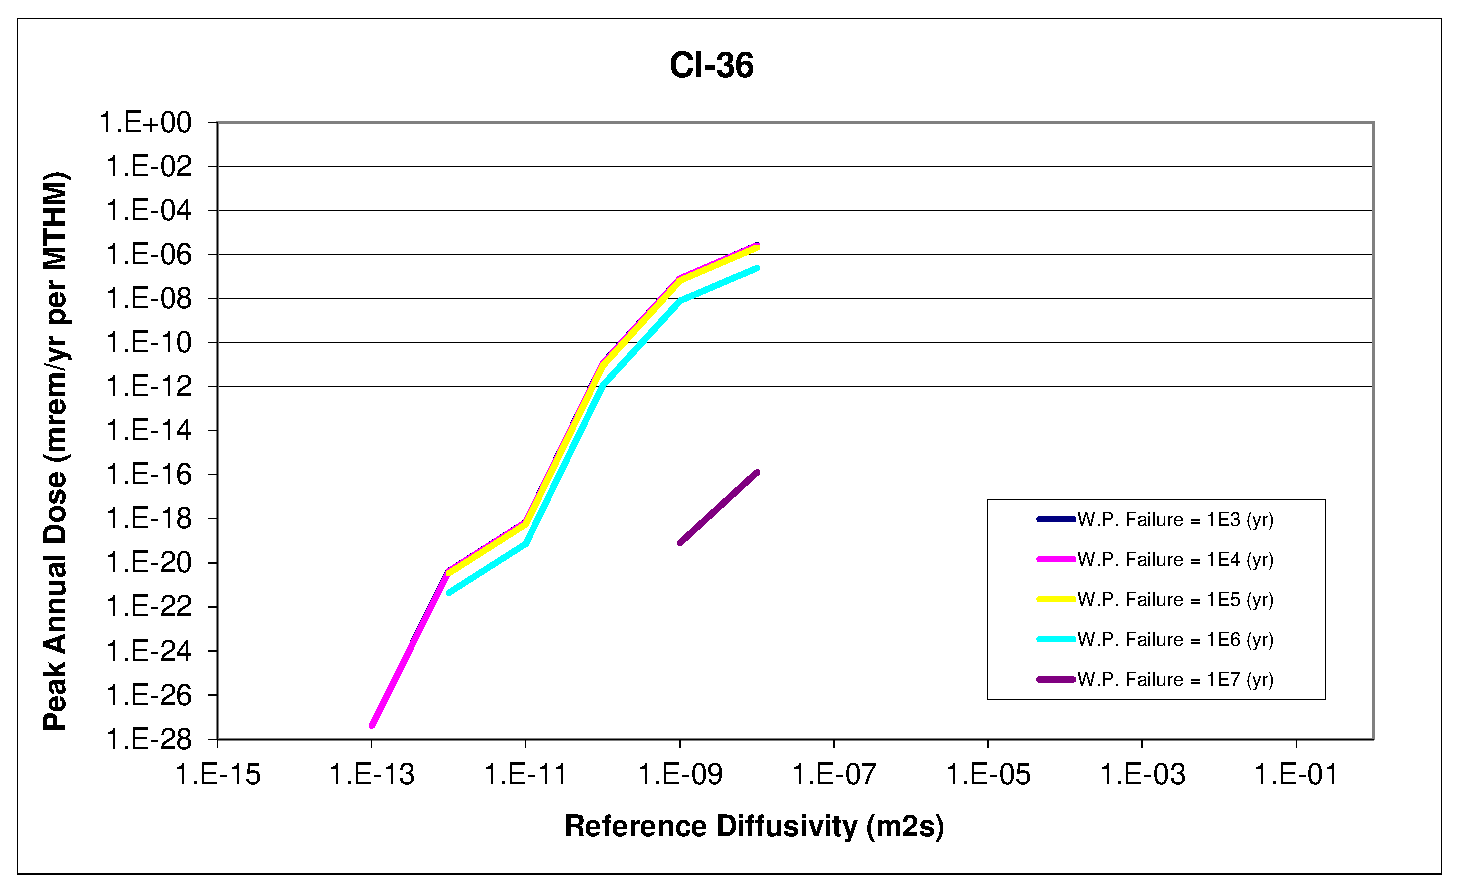
\includegraphics[width=\linewidth]{WPFailExtended/Cl-36.eps}
\caption{$^{36}Cl$ waste package failure time sensitivity. }
\label{fig:WPFailCl36}
\end{figure}
\end{frame}

\begin{frame}[c]
  \frametitle{Case VI : Waste Package Failure Time and Diffusion Coefficient}

\begin{figure}[ht!]
\centering
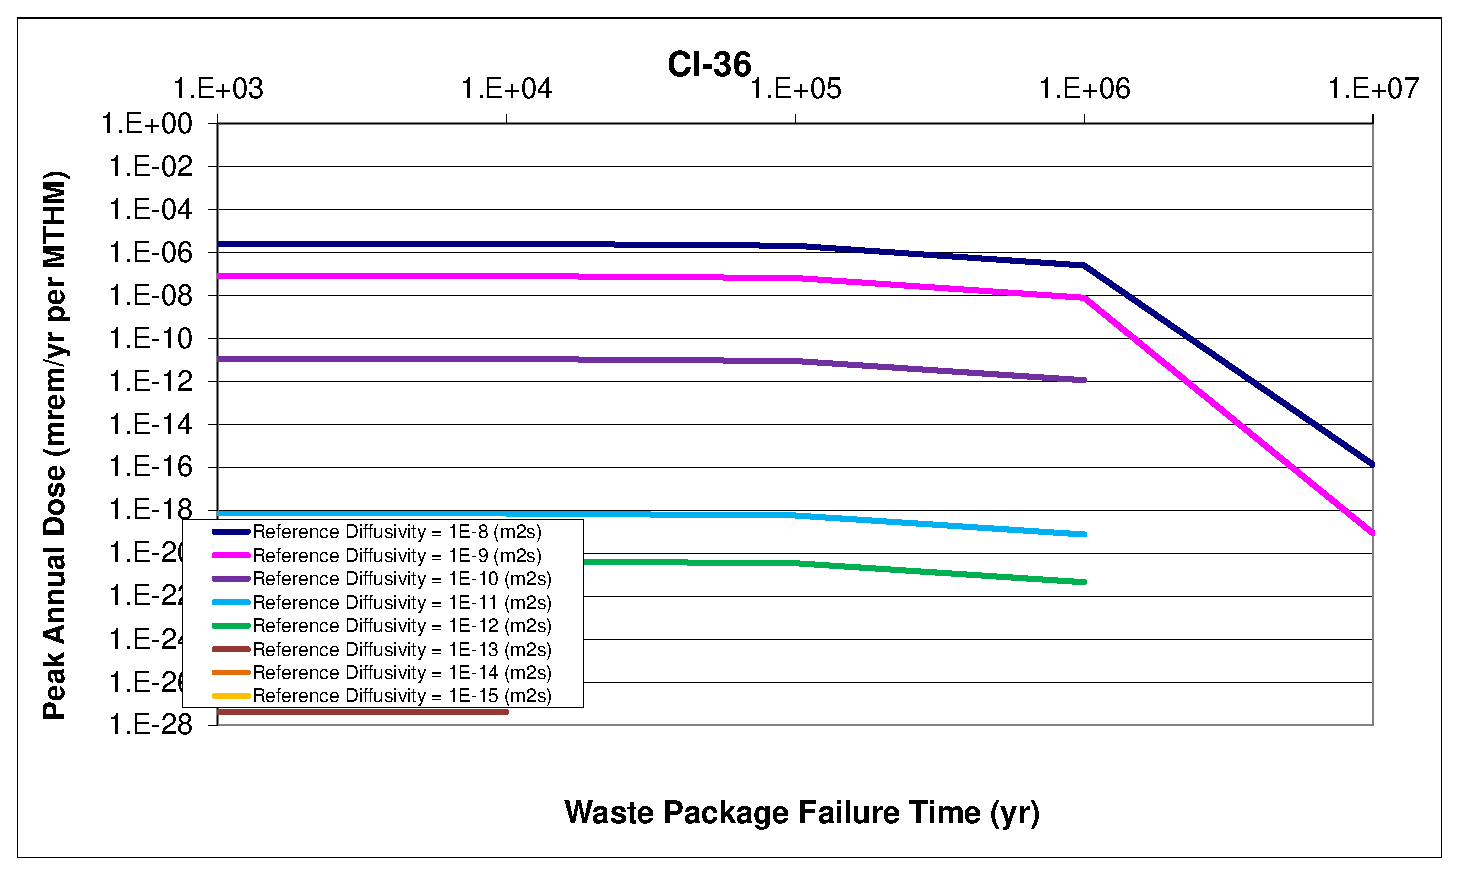
\includegraphics[width=\linewidth]{WPFailExtended/Cl-36-WPFail.eps}
\caption{$^{36}Cl$ waste package failure time sensitivity. }
\label{fig:WPFailPuDaughters}
\end{figure}

\end{frame}

\begin{frame}[c]
  \frametitle{Case VI : Waste Package Failure Time and Diffusion Coefficient}
\begin{figure}[ht!]
\centering
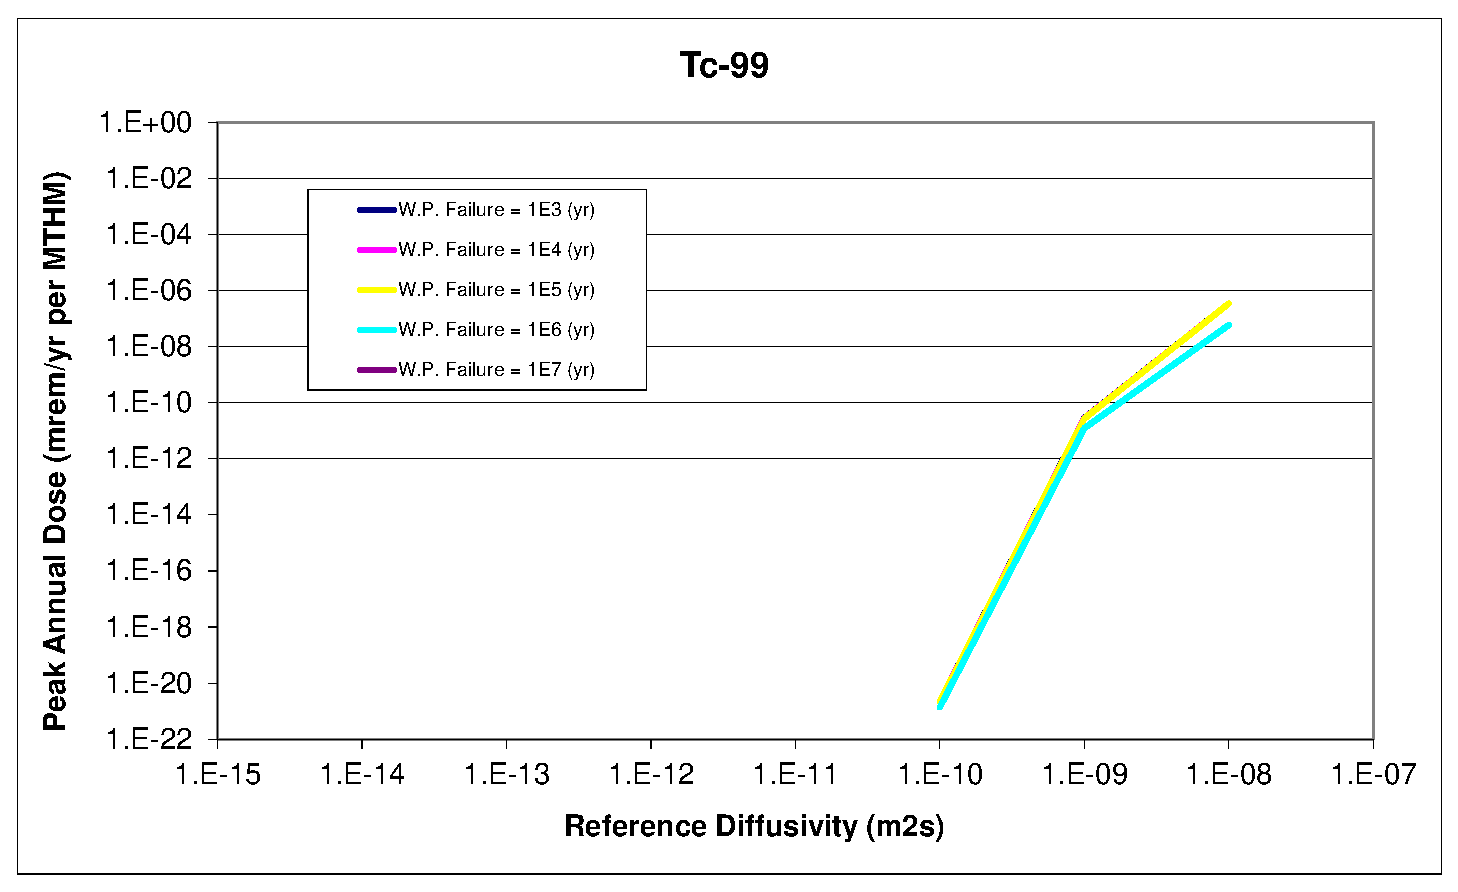
\includegraphics[width=\linewidth]{WPFailExtended/Tc-99.eps}
\caption{$^{99}Tc$ waste package failure time sensitivity. }
\label{fig:WPFailTc99}
\end{figure}
\end{frame}

\begin{frame}[c]
  \frametitle{Case VI : Waste Package Failure Time and Diffusion Coefficient}

\begin{figure}[ht!]
\centering
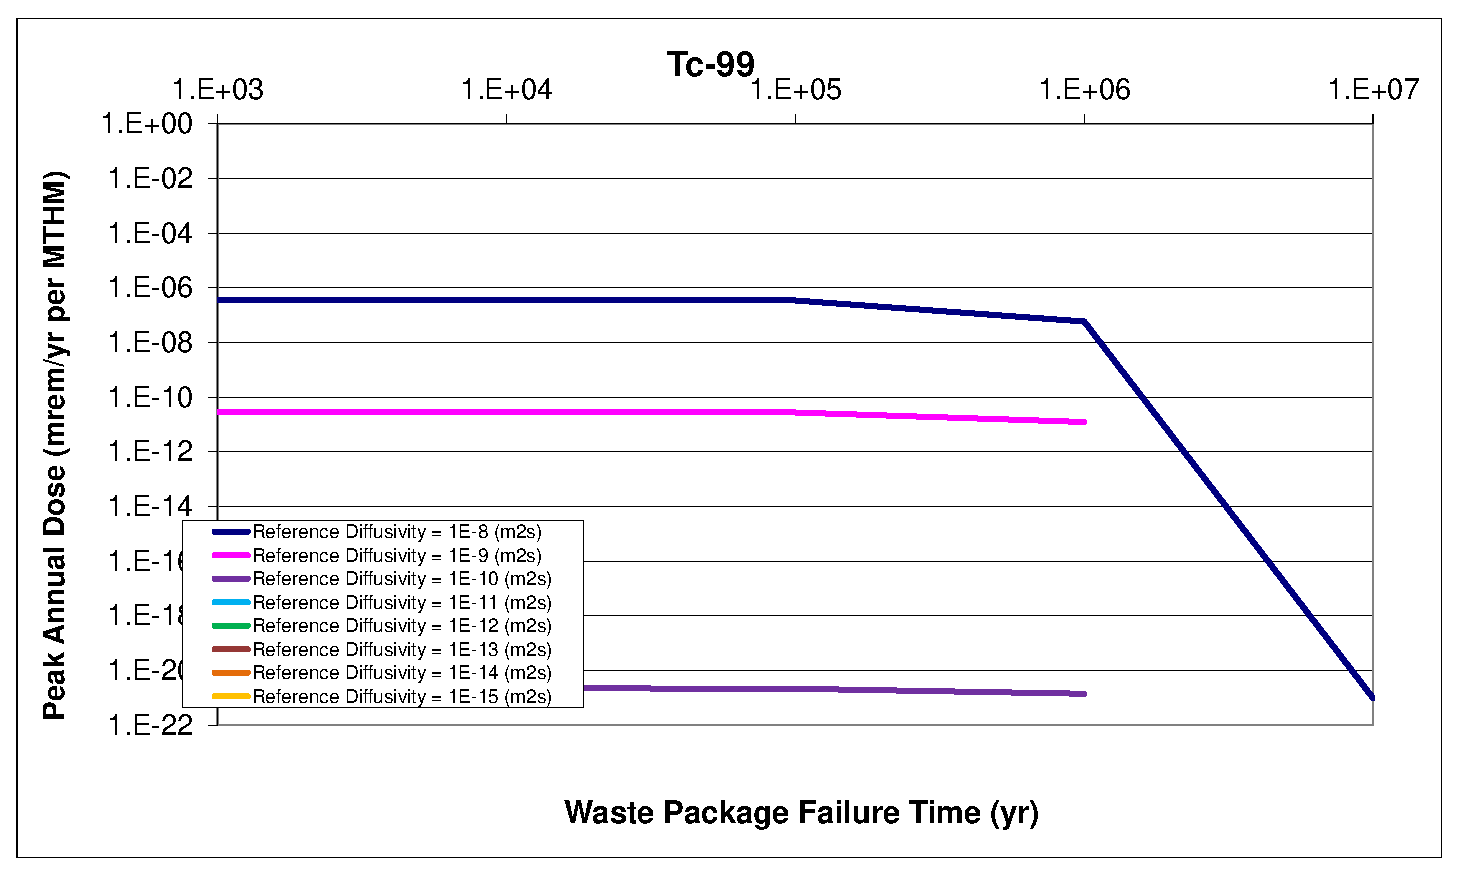
\includegraphics[width=\linewidth]{WPFailExtended/Tc-99-WPFail.eps}
\caption{$^{99}Tc$ waste package failure time sensitivity. }
\label{fig:WPFailTc99}
\end{figure}
\end{frame}

\begin{frame}[c]
  \frametitle{Case VI : Waste Package Failure Time and Diffusion Coefficient}

\begin{figure}[ht!]
\centering
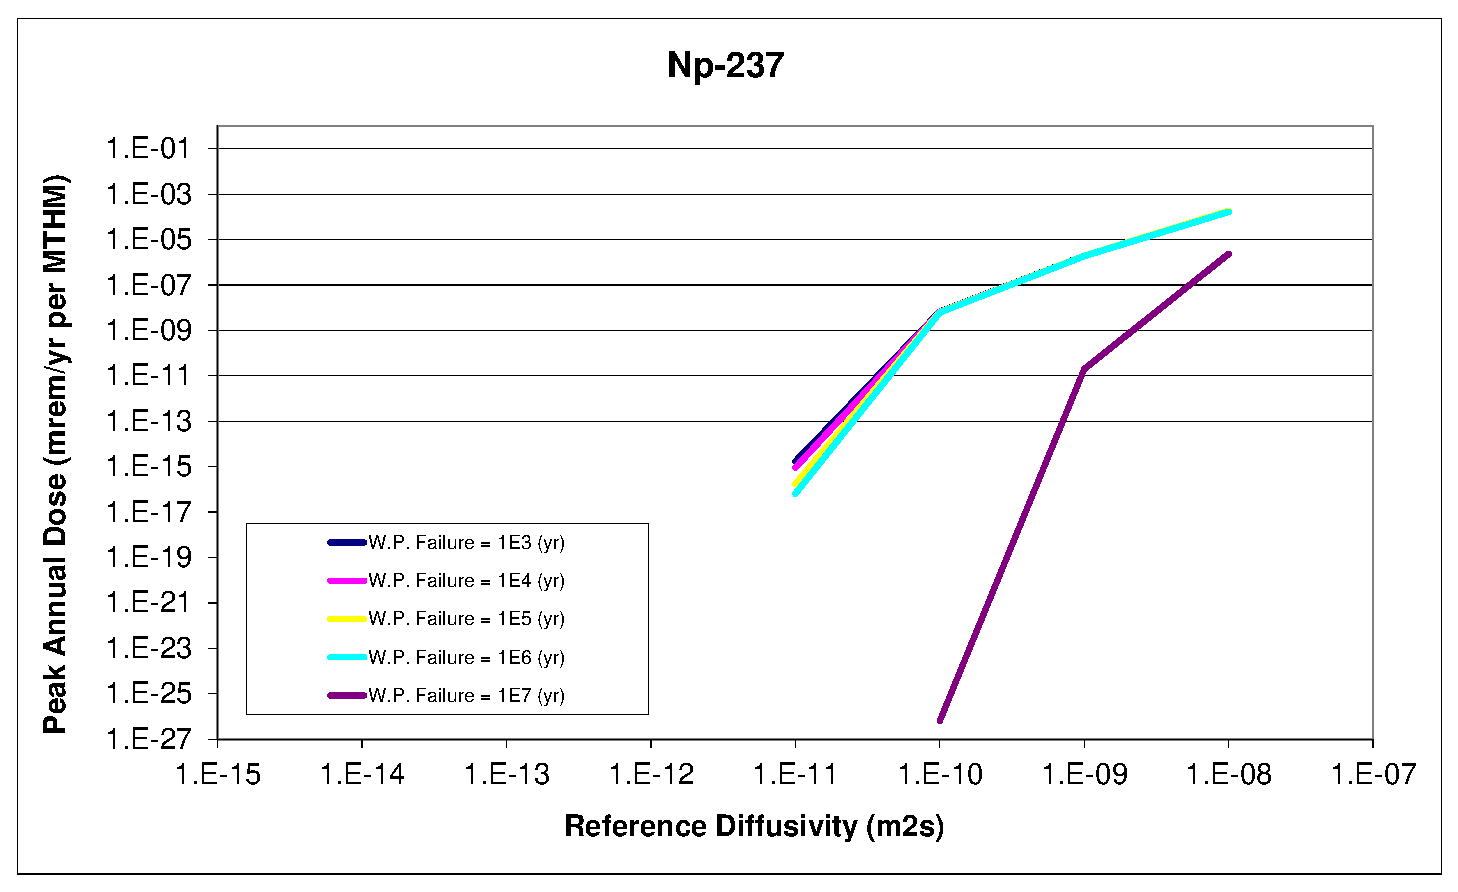
\includegraphics[width=\linewidth]{WPFailExtended/Np-237.eps}
\caption{$^{237}Np$ waste package failure time sensitivity. }
\label{fig:WPFailNp237}
\end{figure}
\end{frame}

\begin{frame}[c]
  \frametitle{Case VI : Waste Package Failure Time and Diffusion Coefficient}

\begin{figure}[ht!]
\centering
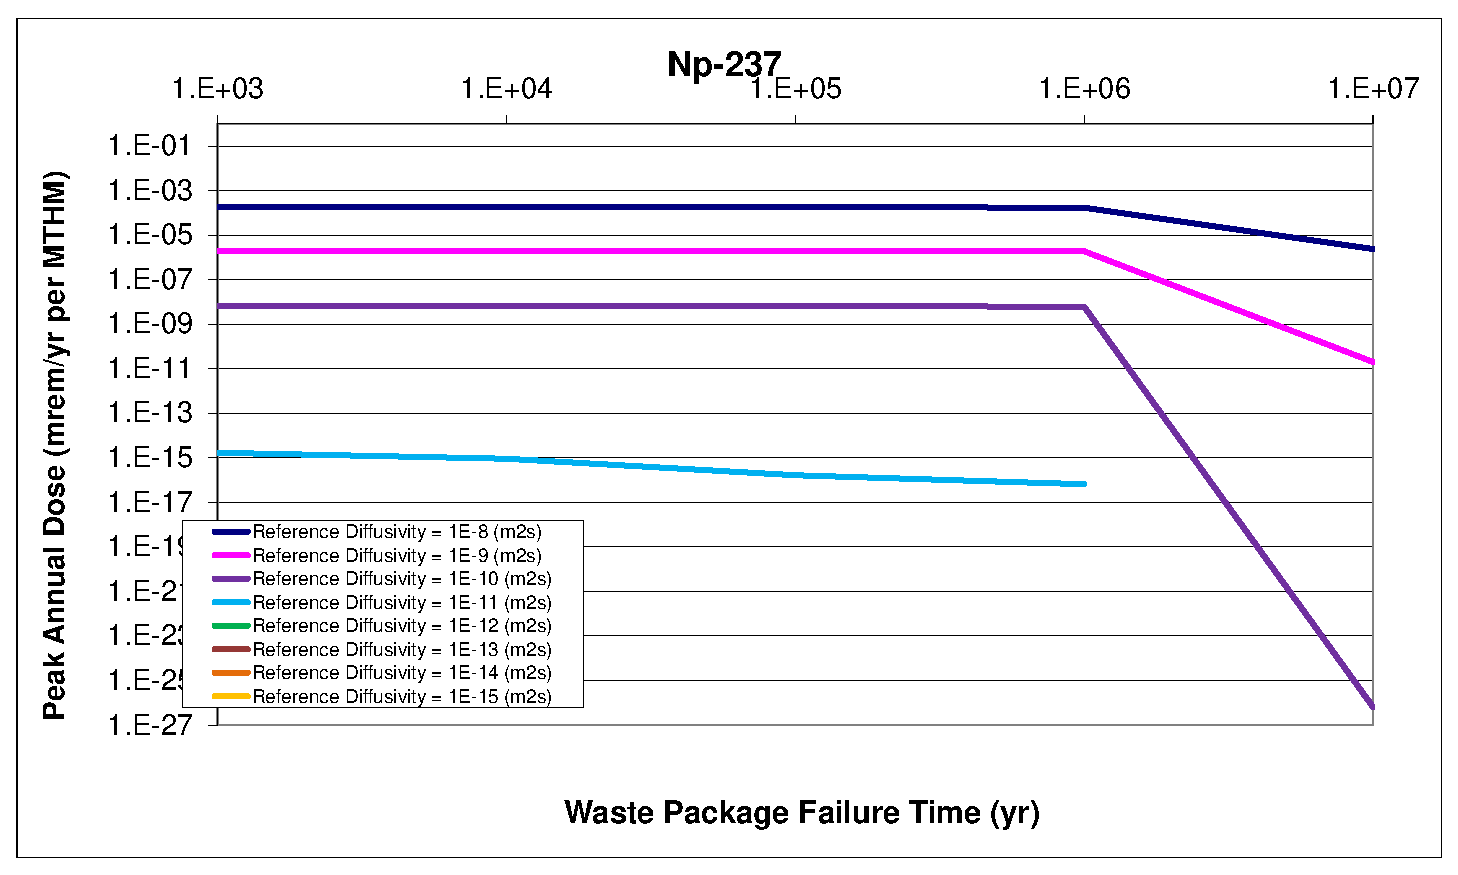
\includegraphics[width=\linewidth]{WPFailExtended/Np-237-WPFail.eps}
\caption{$^{237}Np$ waste package failure time sensitivity. }
\label{fig:WPFailPuDaughters}
\end{figure}
\end{frame}





%%%%%%%%%%%%%%%%%%%%%%%%%%%%%%%%%%%%%%%%%%%%%%%%%%%%%%%%%%%%%%%%%%%%%%%%%%%%%%%%
  
\begin{frame}[c]
  \frametitle{Acknowledgements}
This work is supported by the U.S. Department of Energy, Basic Energy Sciences, 
Office of Nuclear Energy, under contract \# DE-AC02-06CH11357.
\end{frame}


%%%%%%%%%%%%%%%%%%%%%%%%%%%%%%%%%%%%%%%%%%%%%%%%%%%%%%%%%%%%%%%%%%%%%%%%%%%%%%%%}<++>



%%--------------------------------%%
%%--------------------------------%%
\begin{frame}[allowframebreaks]
  \frametitle{References}
  \bibliographystyle{plain}
  {\footnotesize \bibliography{bibliography} }

\end{frame}

%%--------------------------------%%

\end{document}




